%% 明石研究室修士論文テンプレート

\documentclass[a4paper,12pt,titlepage]{jarticle}
\usepackage[dvipdfmx]{graphicx}
\usepackage{color}
\usepackage{amsmath,amssymb,bm}
\usepackage{wrapfig}
\usepackage{url}
\usepackage{afterpage}
\usepackage{ascmac}
\usepackage{array}
\usepackage{geometry}
\usepackage{emathC}
\usepackage{itembkbx}
\usepackage{itembbox}
\usepackage{eclbkbox}
\usepackage{here}
\usepackage{listings, jlisting}
\usepackage{comment}

\renewcommand{\lstlistingname}{リスト}
\lstset{language=c,
  basicstyle=\ttfamily\scriptsize,
  commentstyle=\textit,
  classoffset=1,
  keywordstyle=\bfseries,
  frame=tRBl,
  framesep=5pt,
  showstringspaces=false,
  numbers=left,
  stepnumber=1,
  numberstyle=\tiny,
  tabsize=2
}
\geometry{top=2.5cm,bottom=2.5cm,left=3.1cm,right=3.1cm}
  \makeatletter
  \newcommand{\subsubsubsection}{\@startsection{paragraph}{4}{\z@}%
    {1.0\Cvs \@plus.5\Cdp \@minus.2\Cdp}%
    {.1\Cvs \@plus.3\Cdp}%
    {\reset@font\sffamily\normalsize}
  }
  \makeatother
  \setcounter{secnumdepth}{4}



% 表紙情報
\title{
{\Large 平成27年度 東京理科大学大学院 修士論文 \\[3cm]}
{\Huge レーザー光を用いた\\ハンドジェスチャーの\\拡張現実への応用 \\[3cm]}
{\Large 東京理科大学大学院 理工学研究科 情報科学専攻 \\
明石研究室 修士課程2年\\[2cm]}
}
\author{学籍番号 6313640 \\
渡部 祐太}
\date{}



\begin{document}
% 表紙
\maketitle
% 目次
\tableofcontents



% 本文
\newpage
% 1
\section{序論}

% 1.1
\subsection{背景}
我々は、PCを操作する際にマウス、キーボードを使用する。しかしながら、これらのインターフェースを使いこなすのには時間が必要であり、直感的に扱えるインターフェースとは決して言うことはできない。この問題を解決する一例として、ハンドジェスチャーが挙げられる。この技術により、簡単な操作であれば直感的に行うことができるようになり、より多くの人々が扱うことができる。その一方で、ジェスチャーの種類には限りがあるため、操作が複雑になればなるほど、それを純粋なジェスチャーのみで表現することは難しくなってしまう。そこで、近年ではVR技術と組み合わせることにより、この欠点を補う試みが多々見られる。これにより、多くのシチュエーションに対して、ジェスチャーによる操作を応用することが可能になるため、今後、ハンドジェスチャーはより生活に密接した存在になることが予想される。だが、この進歩の途上には一つの新しい問題が存在する。それは、カメラ等の既存のセンサーが使用できない場所での、ジェスチャーの使用が求められる、というものである。具体例を挙げると、トイレのような倫理的にカメラの使用が憚られる場所がある。この場所では、非接触型インターフェースとして、ハンドジェスチャーの需要が高まると予想されるにも関わらず、カメラをセンサーとして使用した既存の技術は使用することができない。そのような状況への対策として、カメラ以外のセンサーを用いたハンドジェスチャー技術が求められている。

% 1.2
\subsection{目的}
主に二つのことを主眼を置いている。一つ目は、ハンドジェスチャーとVR技術を組み合わせることによって、直感的な操作を行うことができるインターフェースの提案をする。二つ目は、ジェスチャーを認識するセンサーとして、カメラを使用しないことにより、これまで利用できなかったシチュエーションでもジェスチャーを利用可能にする、ということである。

% 1.3
\subsection{構成}
本論文は、全六章から構成される。第二章では、本論文において必要となる技術や用語等を紹介する。第三章では、研究の概要と提案手法を記述する。第四章では、提案したシステムの具体的なアルゴリズムを説明する。第五章では、アルゴリズムを実際にどのように実装したのかを、プログラムを交えつつ説明する。第六章では、システムを動作させた結果を提示する。最後に、第七章では、これらのことを踏まえて、考察、結論等の総括を行う。	% 序論
\newpage
% 2
\section{関連用語}

% 2.1
\subsection{VR}
VR についての説明

% 2.2
\subsection{Unity}
Unity についての説明

% 2.3
\subsection{OpenCV}
OpenCV についての説明	% 類似研究
\newpage
% 3
\section{研究概要}



% 3.1
\subsection{概要}
ハンドジェスチャーを使用する際に用いられるセンサーとして、一般的とされているWebカメラではなく、レーザー光を用いる。このことは、従来ジェスチャーを使用できなかったシチュエーションや場所においても、使用することを可能とする。

具体的なレーザー光の使用方法を説明する。多数のレーザーと、それと同数の受光器を用意して、お互いが対面するように配置することにより、その間を手が遮った際に検出できるようにする。この検出した情報から手のおおよその形状を認識する。予め3Dオブジェクトを配置した、三次元の仮想空間を用意して、そこに取得した手の形状を描画し、3Dオブジェクトを動かすことができるようにする。このことで、レーザー光を用いたデバイスがインターフェースとして使用することができることを証明する。

本研究では、2台のWebカメラを用いて作成したシミュレータデバイスを用意して実験を行う。



% 3.2
\subsection{提案手法}

% 3.2.1
\subsubsection{レーザー光デバイス}
レーザー光を用いたハンドジェスチャーを可能とするため、図3-1のようなデバイスを作成した。

\begin{center}
  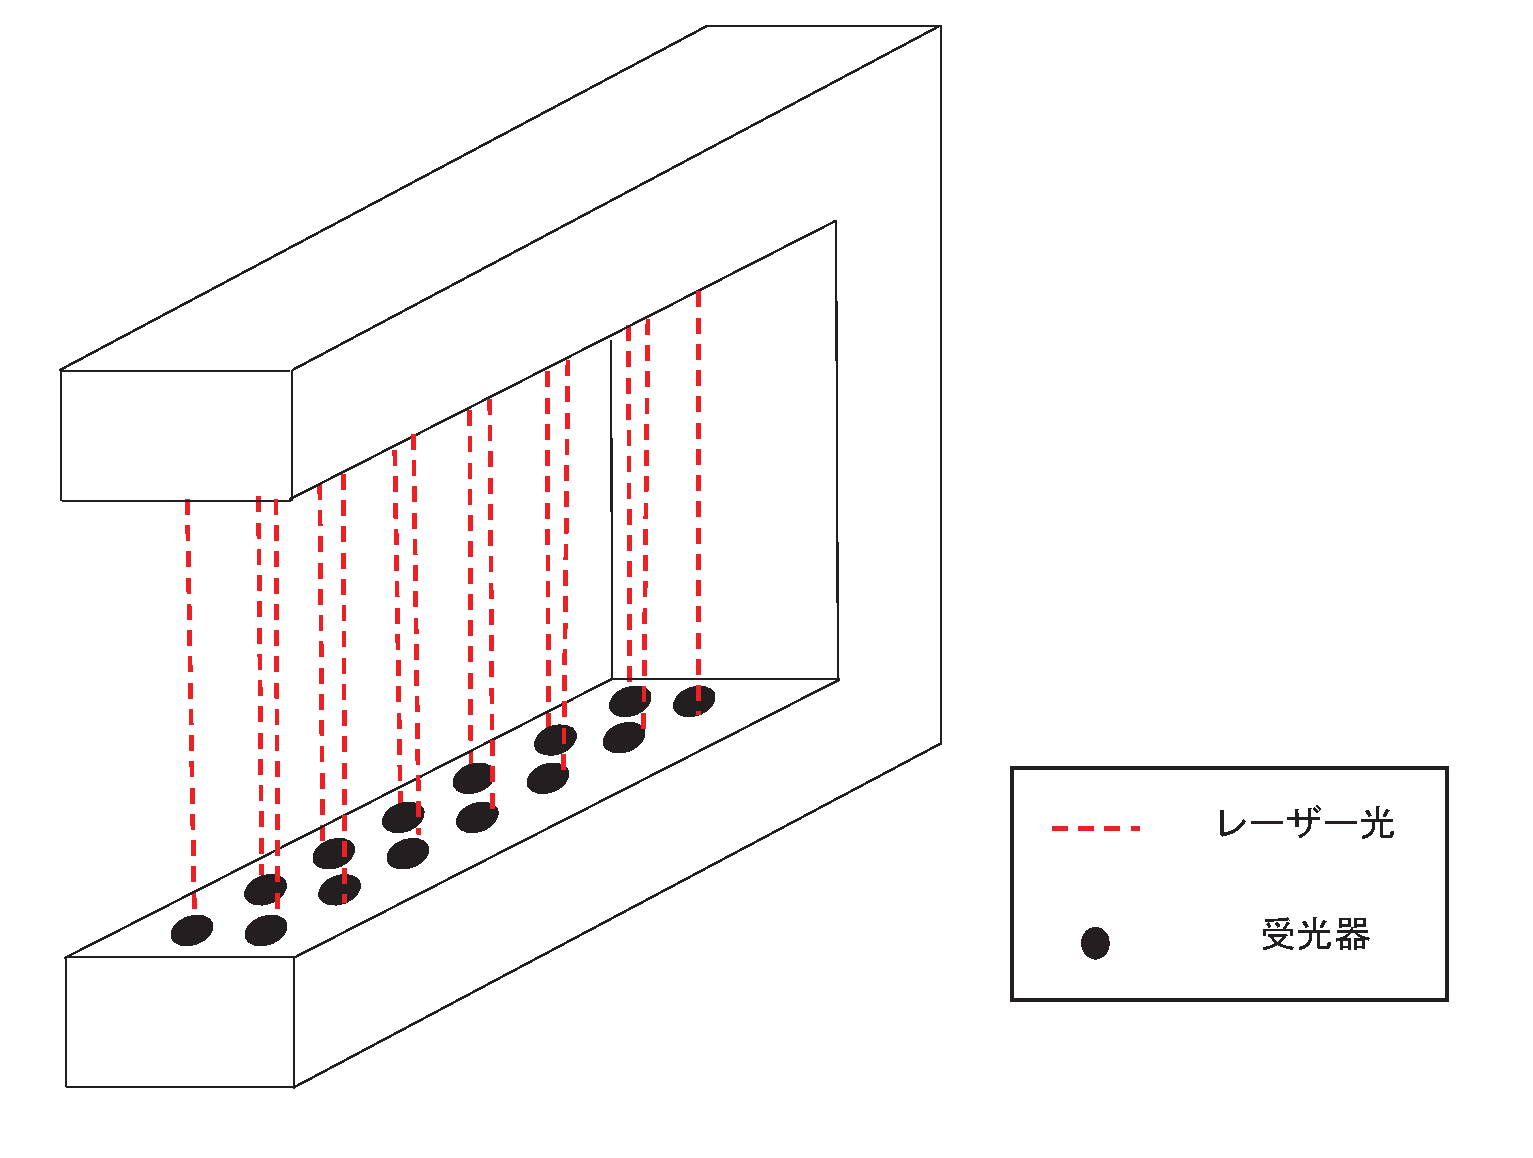
\includegraphics[width=10cm]{RazerDevice_image} \\

 \vspace{1mm}
  図3-1. レーザー光を用いたデバイスのイメージ
\end{center}

デバイスの上部に、計24個のレーザーを設置する。それと対になるように、下部に同数の受光器を設置する。この間を手が通過すると、レーザー光が遮られたことを受光器が検出する。実際に作成したデバイスを用いて、取得した手情報を画像に描画したものを、図3-2に示す。図3-3は使用したデバイスの写真である。

\begin{center}
  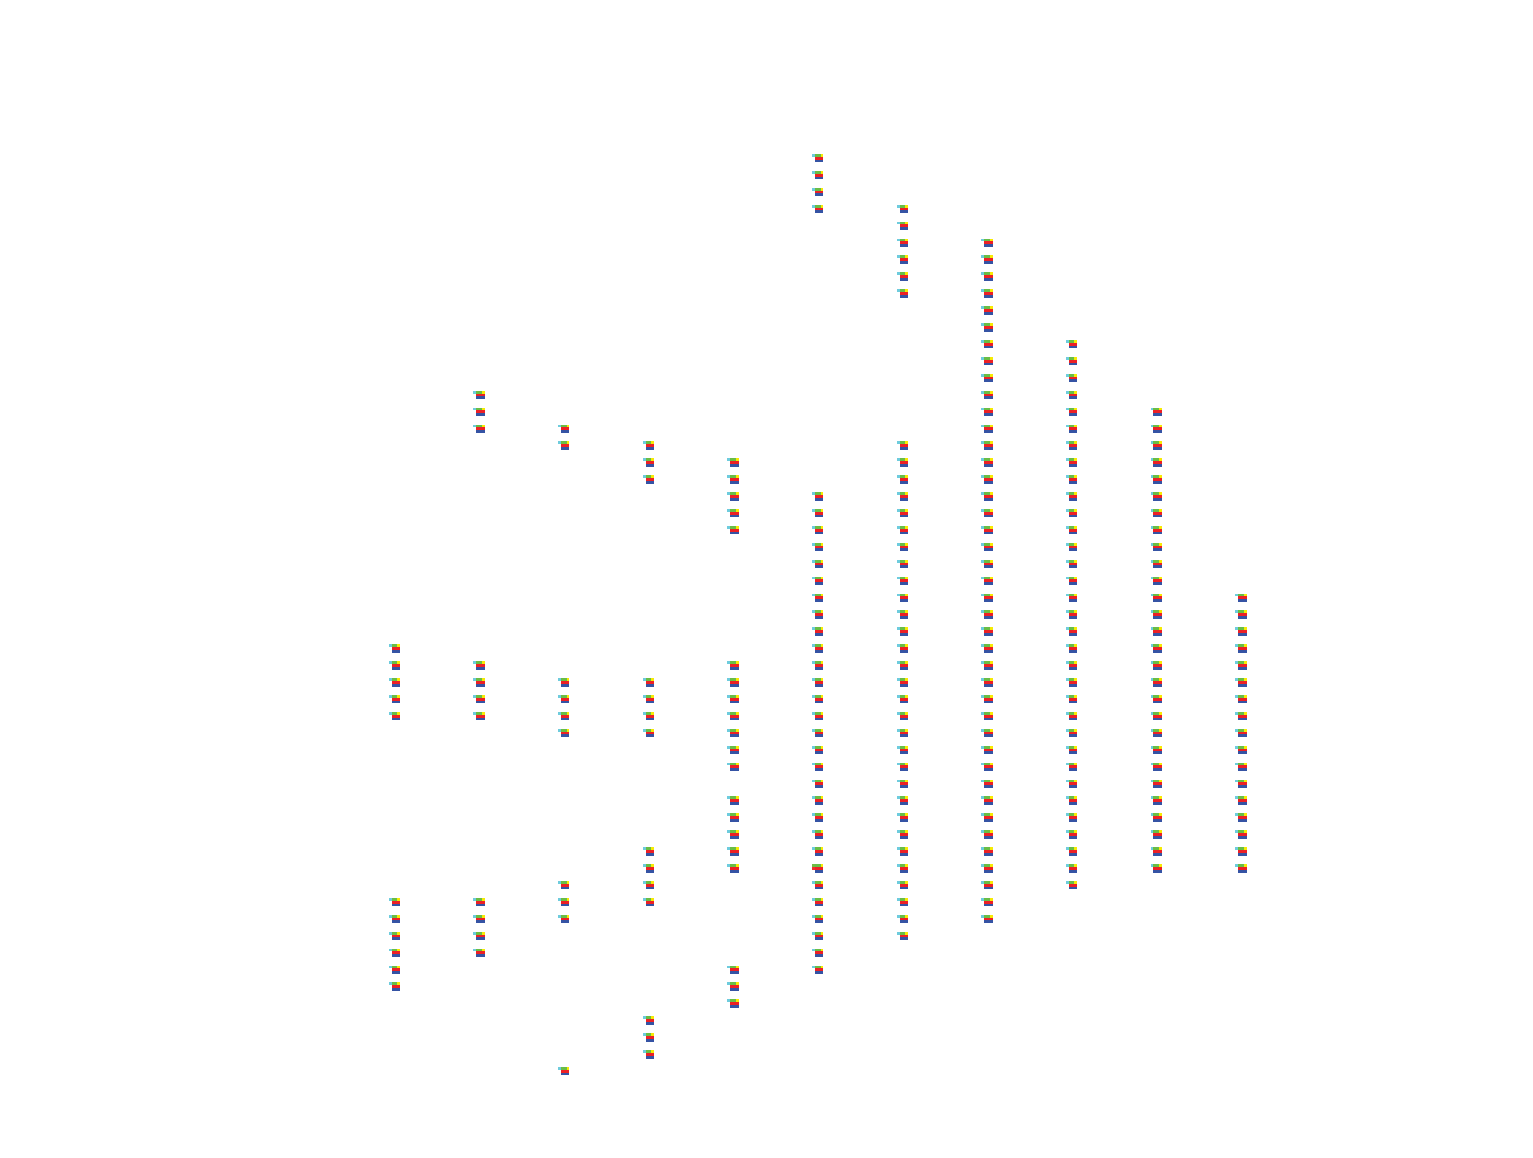
\includegraphics[width=10cm]{RazerDevice_getInfo.eps} \\

 \vspace{1mm}
  図3-2. レーザー光デバイスを用いて実際に得た情報
\end{center}

 \vspace{5mm}

\begin{center}
  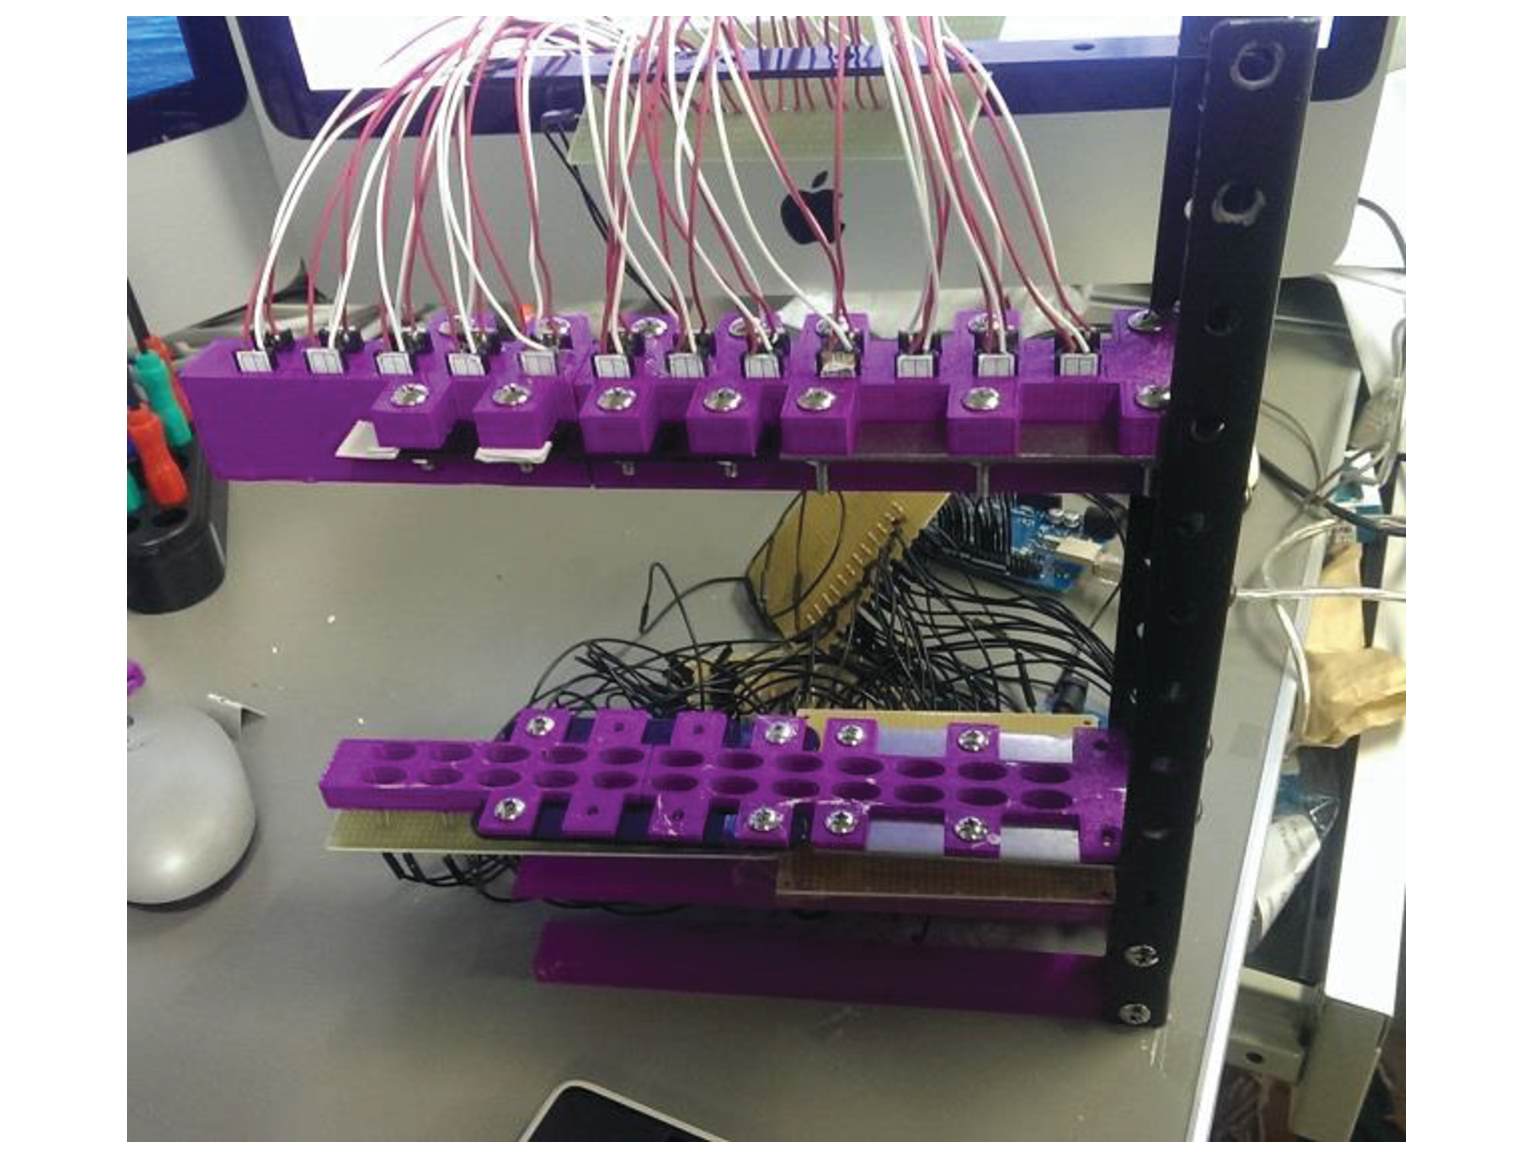
\includegraphics[width=10cm]{RazerDevice_real_color.eps} \\

 \vspace{1mm}
  図3-3. 実際に作成したレーザー光デバイス
\end{center}

図3-2より、レーザー光を用いた手の形状を認識が可能であることが伺える。しかしながら、このデバイスには問題が存在する。それは、レーザー数が足りないということである。手の情報を得るためには、スキャナーのように手を固定した形で通過させる必要がある。この制約は、動的な手情報を得ることができないことを示している。つまり、VRと組み合わせた直感的なハンドジェスチャーインターフェースを作ることは不可能である。だが、図3-2の結果から、認識したい物体の範囲より広くレーザーを設置することが出来れば、動的に手情報を得ることができると推測される。% このデバイスのイメージ用意してもいいかも
このことを踏まえて、レーザー光の代わりにWebカメラを用いたシミュレータデバイスを作成した。

% 3.2.2
\subsubsection{Webカメラを用いたシミュレータデバイス}
図3-4は、レーザー光の代わりにWebカメラを用いたシミュレータデバイスのイメージとなる。側面が一つ空いているボックスの上面と側面に対して、図3-4のようにWebカメラを設置する。レーザー光による検出を再現するために、Webカメラから得られた映像に対して、一定間隔毎に情報を取得する座標を設けることとする。カメラの対面に青いスクリーンを貼り付けることによって、間を青以外の物体が遮った時に、それを検出できるようにする。実際にボックスの中に手を入れて、取得した情報を図3-5に示す。図3-5は図3-4の上部に設置したWebカメラから取得した情報である。同様の手法で、横のWebカメラからも同時に情報を取得する。縦、横の二つの画像から手情報を三次元空間に構築して、同空間に生成したオブジェクトを動かすことにより、直感的なジェスチャーを可能にするための道筋を示す。図3-6は実際に作成したシミュレータデバイスである。

\begin{center}
  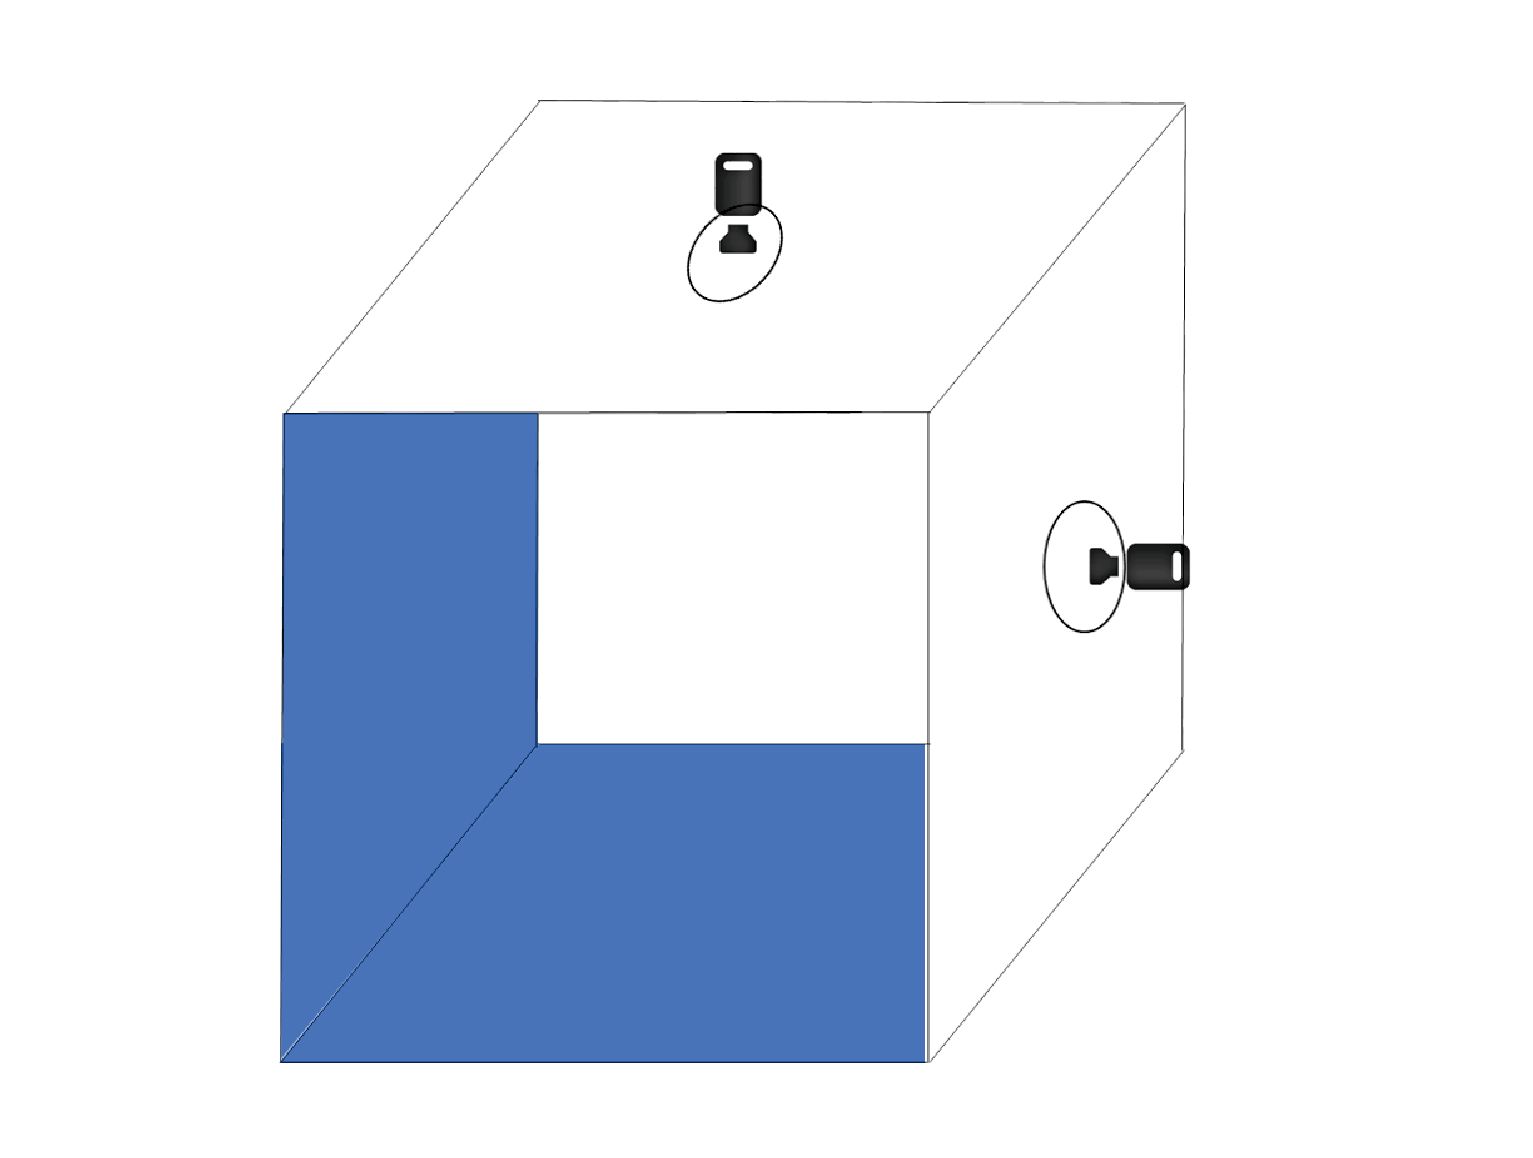
\includegraphics[width=10cm]{Simulator_image.eps} \\

 \vspace{1mm}
  図3-4. Webカメラを用いたシミュレータデバイスのイメージ
\end{center}

\begin{center}
  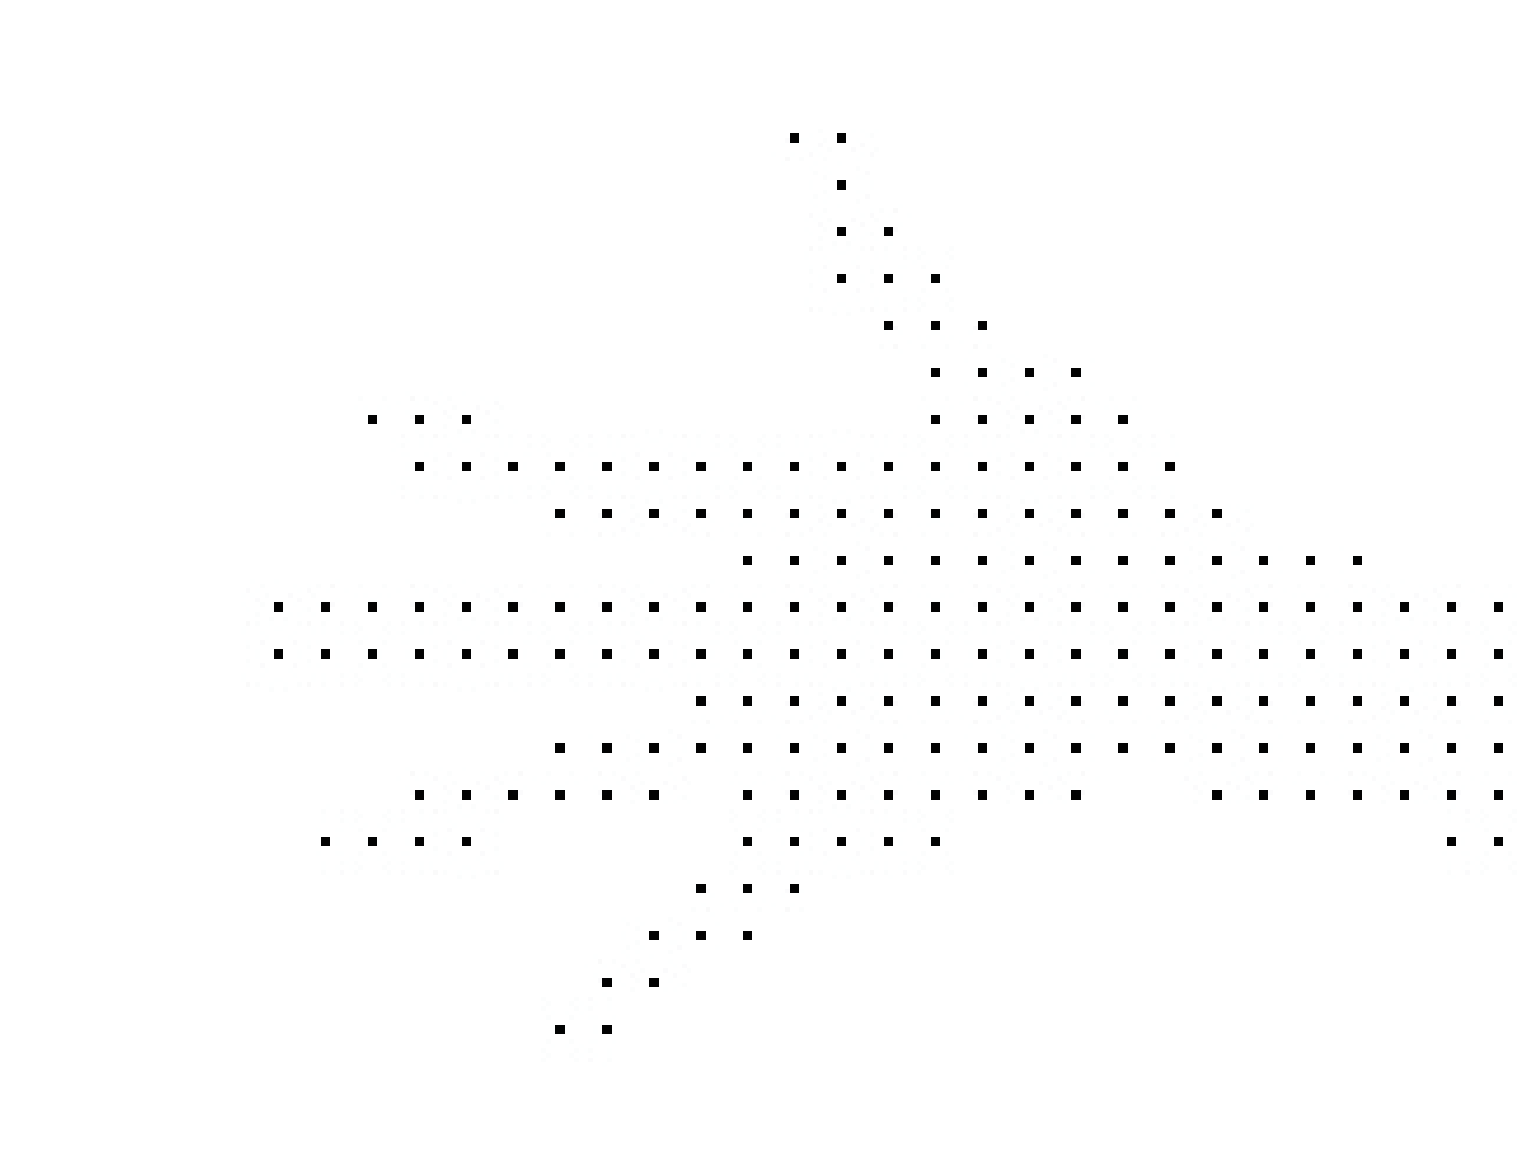
\includegraphics[width=10cm]{Simulator_getInfo.eps} \\

 \vspace{1mm}
  図3-5. シミュレータデバイスから得られた情報
\end{center}

 \vspace{10mm}
\begin{center}
  \includegraphics[width=10cm]{Simulator_real_color.eps} \\

 \vspace{1mm}
  図3-5. 実際に作成したシミュレータデバイス
\end{center}

% 3.2.3
\subsubsection{3Dオブジェクトと手情報の接触判定}
オブジェクトが存在する三次元空間に、正方格子点が存在すると考える。それらの点がオブジェクトの内部にあるのか、外部にあるのかを判定する。その判定結果と手情報を比較することによって、3Dオブジェクトを動かせるようにする。判定する方法について詳しく述べる。三次元空間を一定間隔の層に分ける。各階層毎に内部外部判定を行うことで、擬似的に三次元オブジェクトに対して内部外部判定を行うことができる。各階層毎の内部外部判定には、外積計算と Cauchy の積分定理を組み合わせた手法を用いる。ここで、外積計算による判定方法と、 Cauchy の積分定理による判定方法について説明を行う。一般的な特徴として、外積計算による方法は、くぼみや穴などを有するドーナッツ型の図形に対する内部外部判定が不利であり、かつ複雑形状の図形において、境界線から離れた内部で判定が困難である。Cauchy の積分定理による方法は、くぼみや穴などを有するドーナッツ型の図形に対する内部外部判定が有利である一方で、複雑形状の図形において、境界線付近での判定に難があるというデメリットが存在する。そこで本研究では、 Cauchy の積分定理の弱点を、外積計算による方法で補う手法を取る。






















	% 研究概要
\newpage
% 4
\section{アルゴリズム}
どのような流れで、プログラムが動作しているのか説明を行う。大まかな流れに分けると次のようになる。

\begin{enumerate}
 \item デバイスに設置した二台の'Webカメラから、それぞれ映像をキャプチャする。これらのカメラは縦、横に設置される。
 \item それぞれのキャプチャした画像上に、正方格子点が存在すると考える。点と重なる画素について、青色かどうか判定して結果を取得する。青色でない場合、何かしらの物体が存在すると判断する。
 \item 縦、横、それぞれの結果を組み合わせることで、3次元のデータを生成する。
 \item 三次元空間に、正方格子点が存在すると考える。この空間には、あらかじめデータを入力した三次元オブジェクトを配置している。すべての格子点について、このオブジェクトの内部にあるか外部にあるのかを判定して結果を取得する。
 \item 3で得た物体情報が格納された三次元データと、5で得た内部外部判定が格納された三次元データを比較する。3で物体が存在すると判断された点と、4で内部と判定された点が重なっている場合、物体はオブジェクトの内部に存在すると判断する。
 \item 物体がオブジェクト外部に出るように三次元オブジェクトを移動させる。
\end{enumerate}
 
本章では、2、3、4についてより詳細な説明を行う。

% 4.1
\subsection{カメラ画像からの物体データの取得}
縦に設置したWebカメラから得た画像について述べる。まず、Webカメラから取得した画像はRGB色空間での表現となっているため、特定の色が抽出しやすいHSV色空間への変換を行う。

 \vspace{5mm}
\begin{minipage}{0.5\hsize}
  \begin{center}
   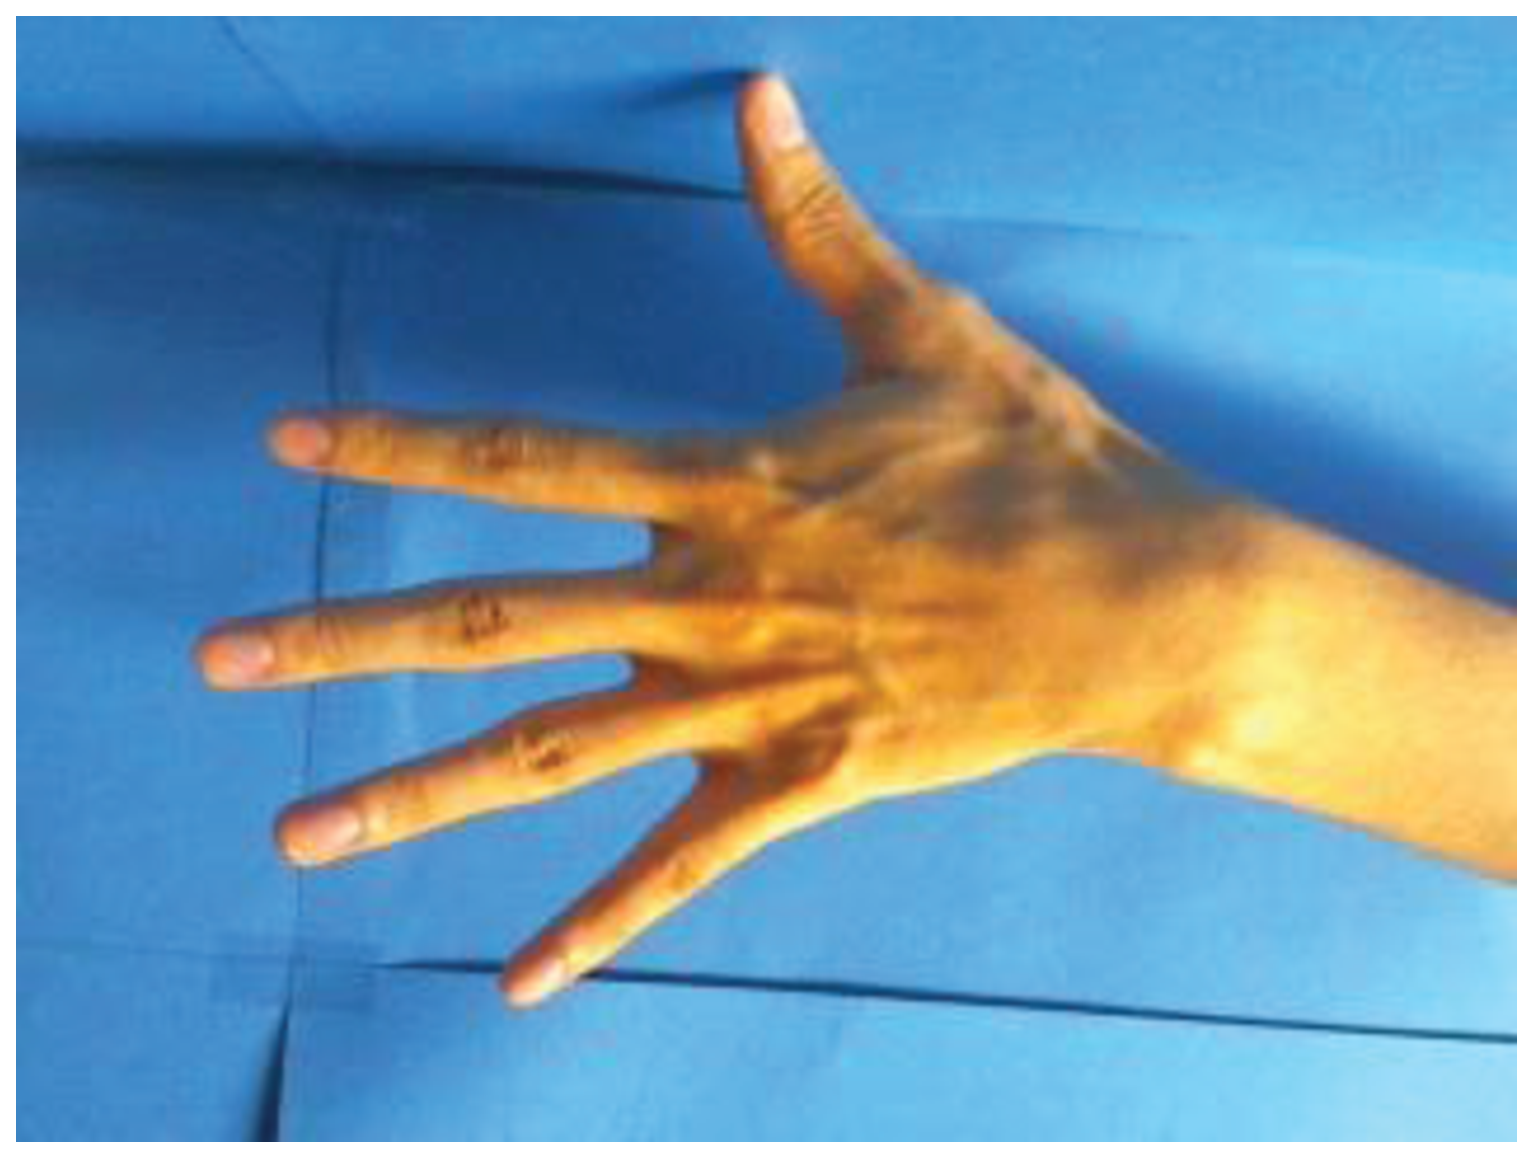
\includegraphics[width=70mm]{Simulator_getPic.eps}
   図4-1. RGB空間での表現
  \end{center}
  \label{fig:one}
 \end{minipage}
 \begin{minipage}{0.5\hsize}
  \begin{center}
   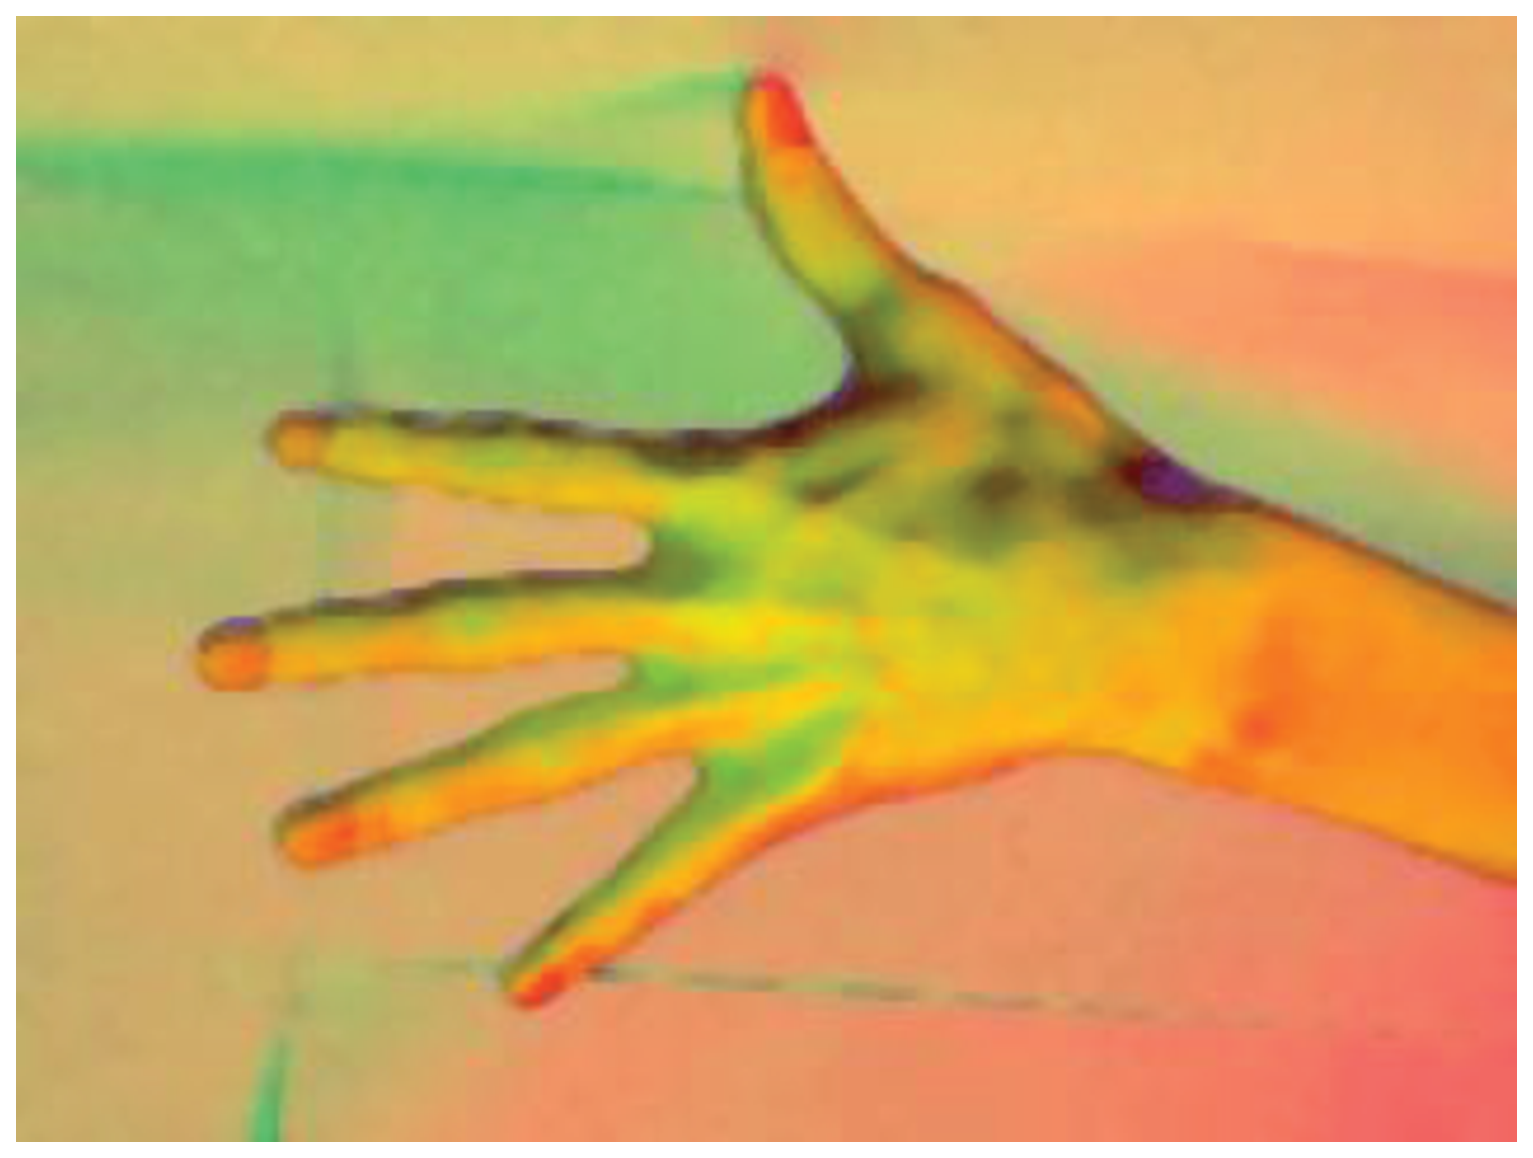
\includegraphics[width=70mm]{Simulator_hsv.eps}
   図4-2. HSV空間での表現
  \end{center}
  \label{fig:two}
 \end{minipage}
 
図4-1はRGB色空間で表現した画像、図4-2はHSV色空間で表現した画像となっている。変換後の画像上で、正方格子点を考える。格子点を画像上に可視化したものが図4-3となる。

\begin{center}
  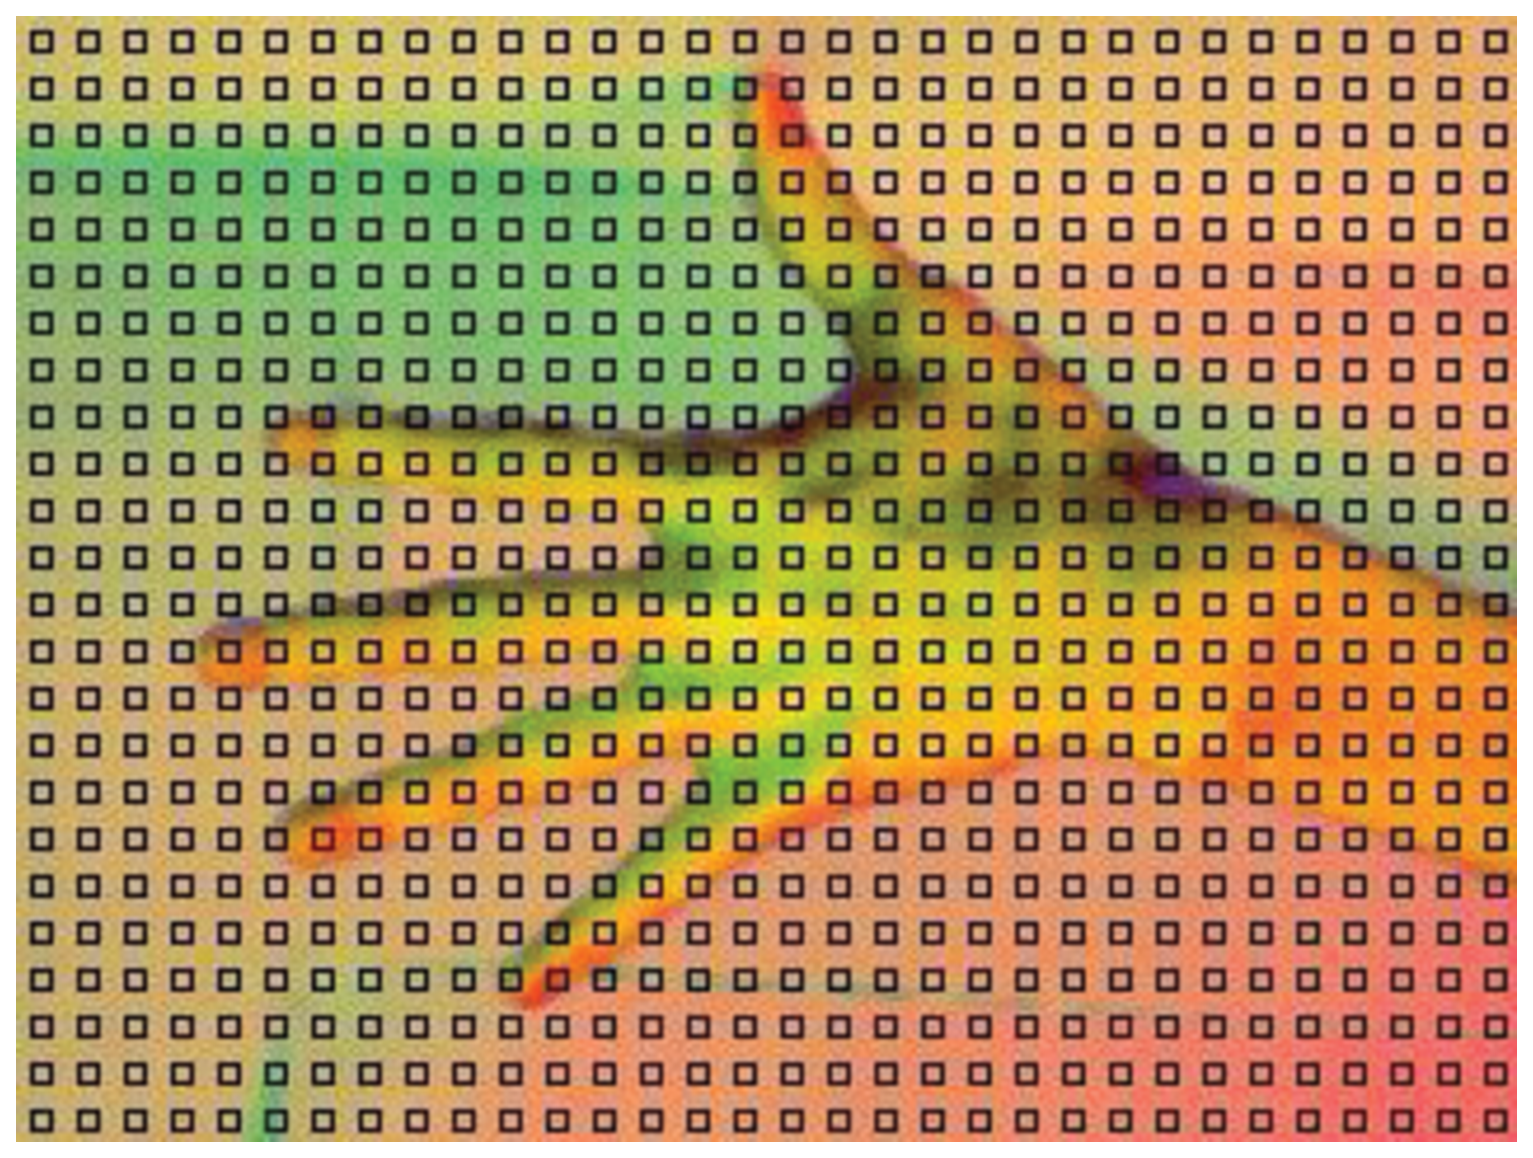
\includegraphics[width=10cm]{Simulator_grid.eps} \\
 \vspace{1mm}
  図4-3. 格子点のイメージ
\end{center}

これらの格子点と重なっている画素について、青色かどうかを判定する。図の4-4は、青色ではない部分を描画したものである。この一連の流れで、レーザー光を用いた際と同じデータを取得することができる。これを横についても、同じことを行う。

\begin{center}
  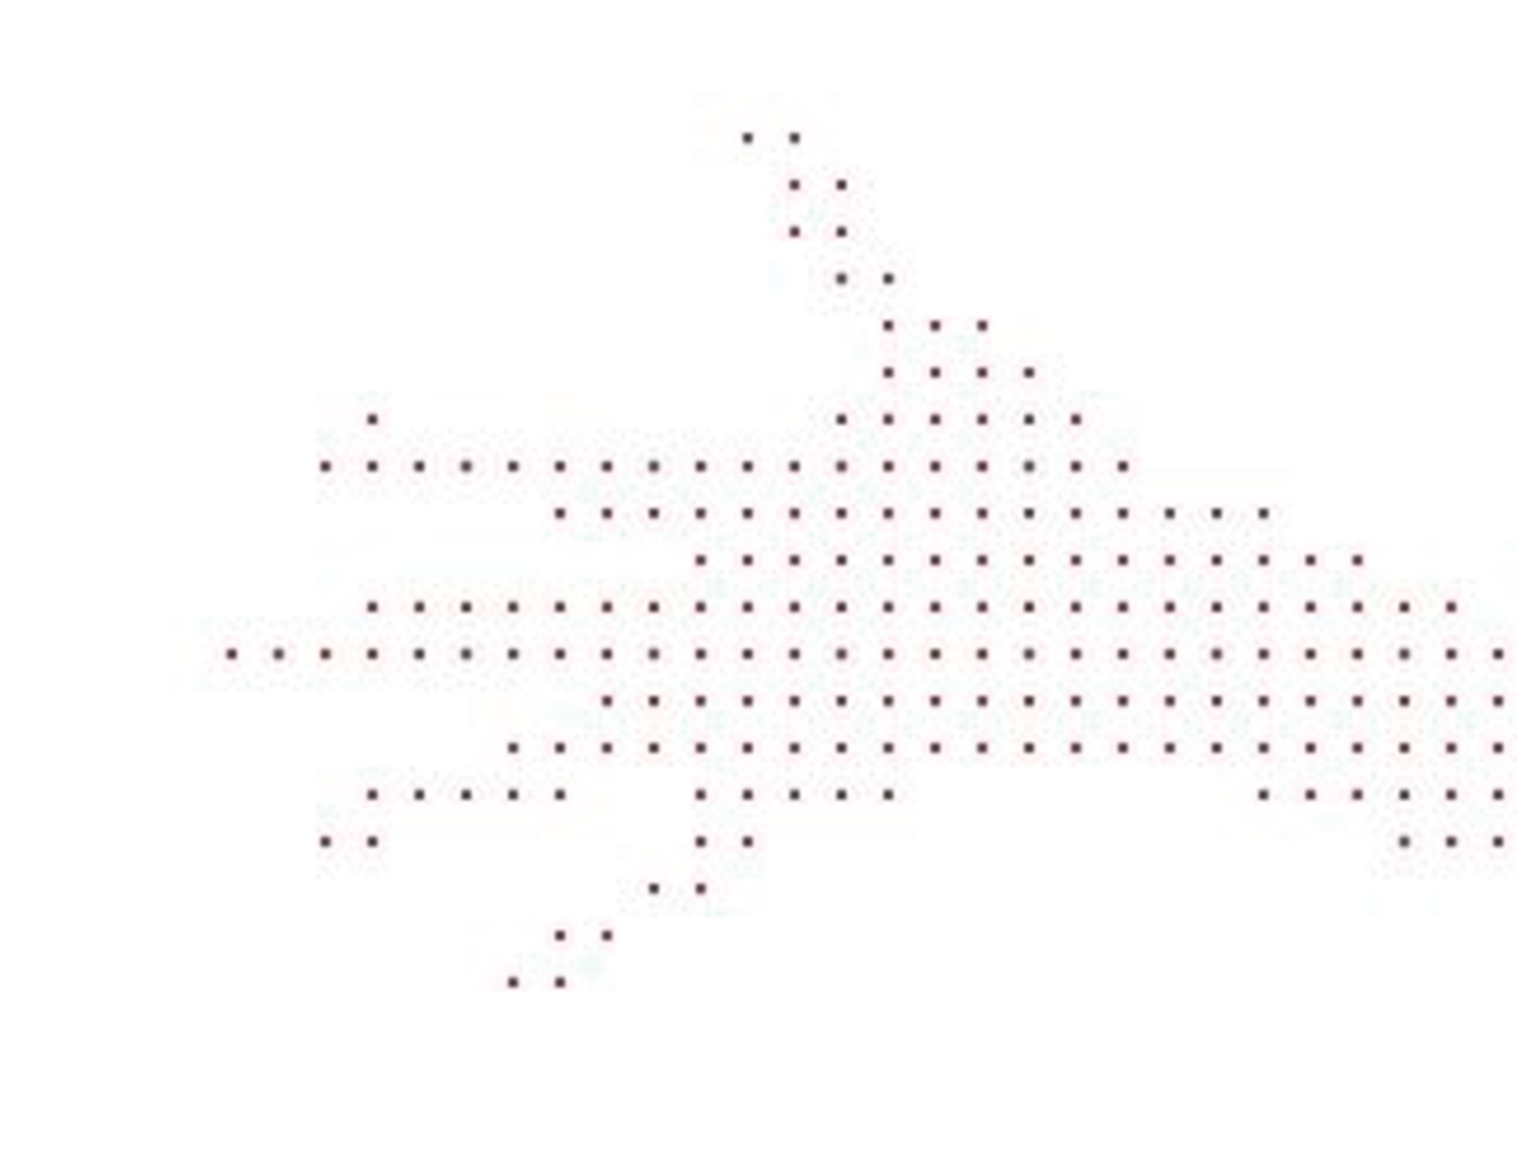
\includegraphics[width=10cm]{Simulator_data.eps} \\
 \vspace{1mm}
  図4-4. 青色ではない部分を描画
\end{center}



\newpage
% 4.2
\subsection{二次元物体データから三次元データを生成}
Webカメラから取得したデータから三次元データを生成する。図4-5、図4-6はそれぞれ縦に設置したカメラ、横に設置したカメラから得たデータとなっている。

 \vspace{5mm}
\begin{minipage}{0.5\hsize}
  \begin{center}
   
\includegraphics[width=70mm]{Simulator_data_h.eps}
   図4-5. 縦に設置したカメラから得たデータ
  \end{center}
  \label{fig:one}
 \end{minipage}
 \begin{minipage}{0.5\hsize}
  \begin{center}
   
\includegraphics[width=70mm]{Simulator_data_v.eps}
   図4-6. 横に設置したカメラから得たデータ
  \end{center}
  \label{fig:two}
 \end{minipage}
 
 始めに、横のカメラから得たデータを元に、Y=0から物体が存在するという情報があるか検索する。存在する情報が発見された時、Xの値を一旦保存する。縦のカメラから得たデータにおいて、先ほど保存したXの値を用いて、物体が存在する情報がないのか検索する。存在する情報が発見された時、Zの値を保存する。この時の、X、Y、Zには物体が存在すると判定する。これをすべてのX、Y、Zについて繰り返し行うことで、三次元のデータを生成する。実際に、図4-5、図4-6から生成した三次元のデータが、図4-7となる。
 
\begin{center}
  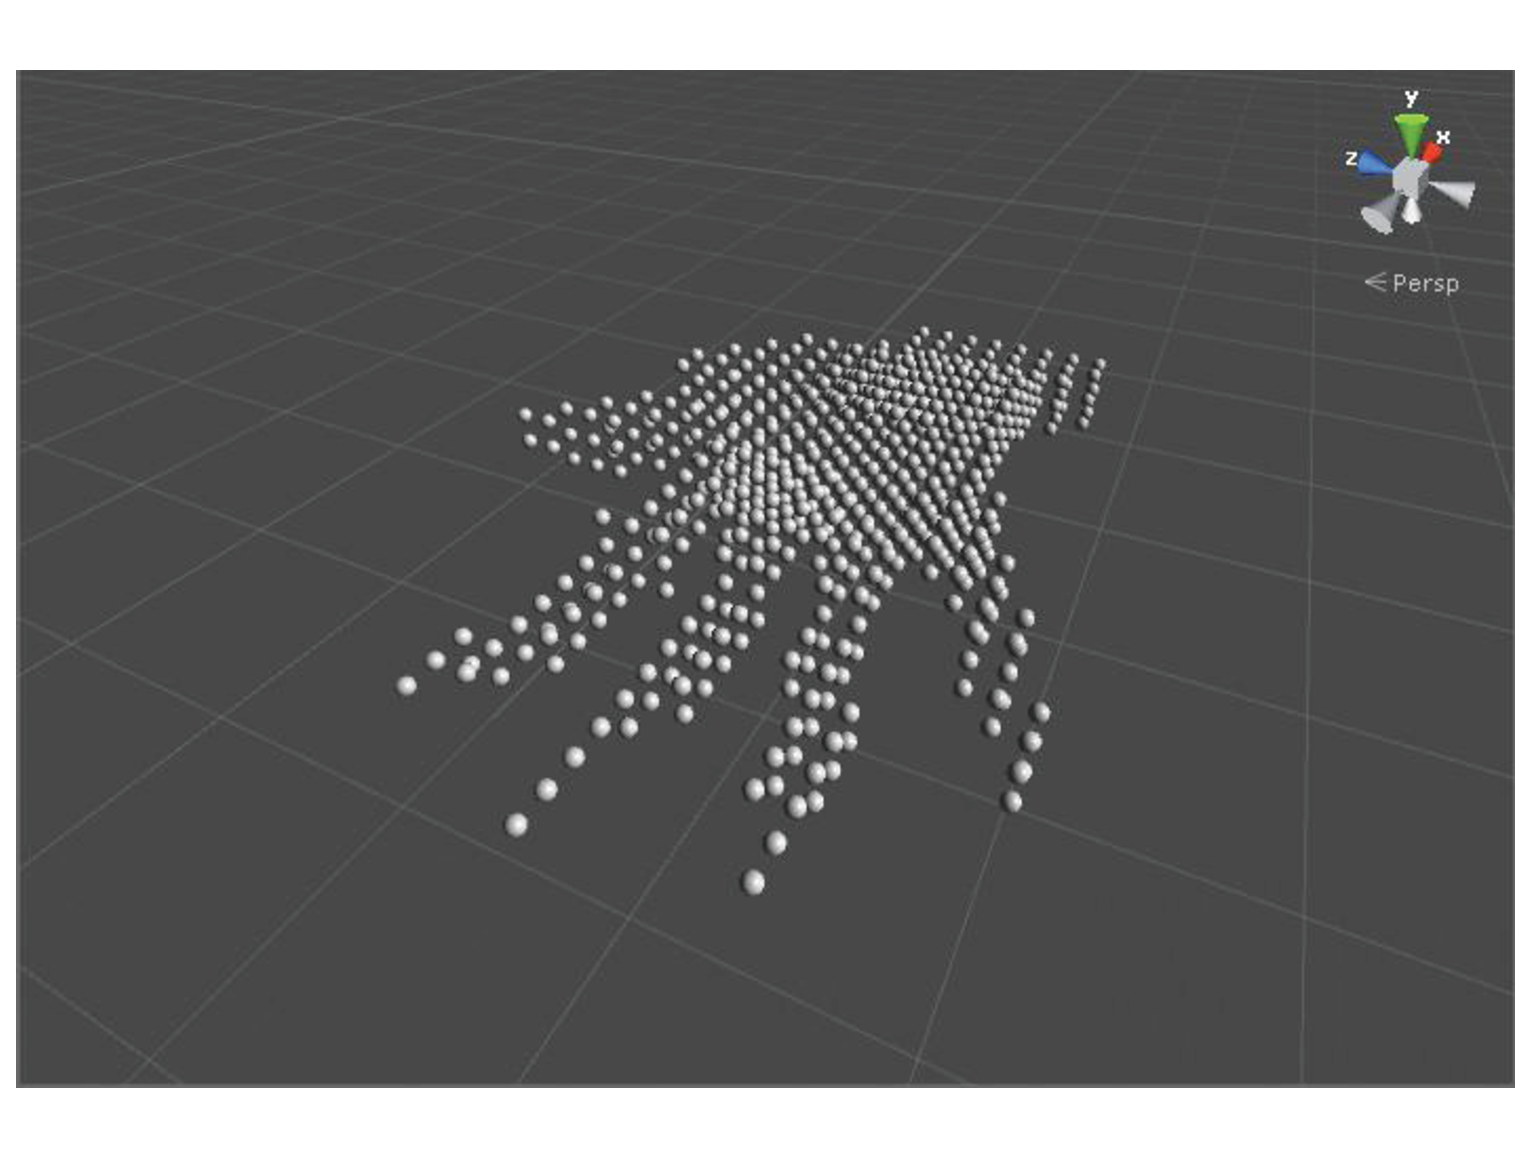
\includegraphics[width=10cm]{Simulator_data_3d.eps} \\
 \vspace{1mm}
  図4-7. 生成した三次元データ
\end{center}



\newpage
% 4.3
\subsection{格子点の内部外部判定}
外積計算による方法と、 Cauchy の積分定理を組み合わせた手法によって、内部外部判定を行うことは既に前章にて記述した。具体的には、外積計算による方法を改良し、図形の境界線付近での内部外部判定を強化したうえで、二つの手法を組み合わせる。まず始めに、外積による計算方法について述べる。既存の方法では、調査点Pと多角形の輪郭を構成する2点 $z_k,z_{k+1}$ の合計三点を用いて計算を行っている。改良版は、調査点Pと輪郭を構成する三点 $z_{k-1},z_k,z_{k+1}$ の合計四点を用いて計算を行う。この改良版の外積計算について、詳しく説明する。

\subsubsection{$z_{k-1},z_k,z_{k+1}$ の三点が、この順番で左回りに三角形を構成している場合}

\begin{center}
  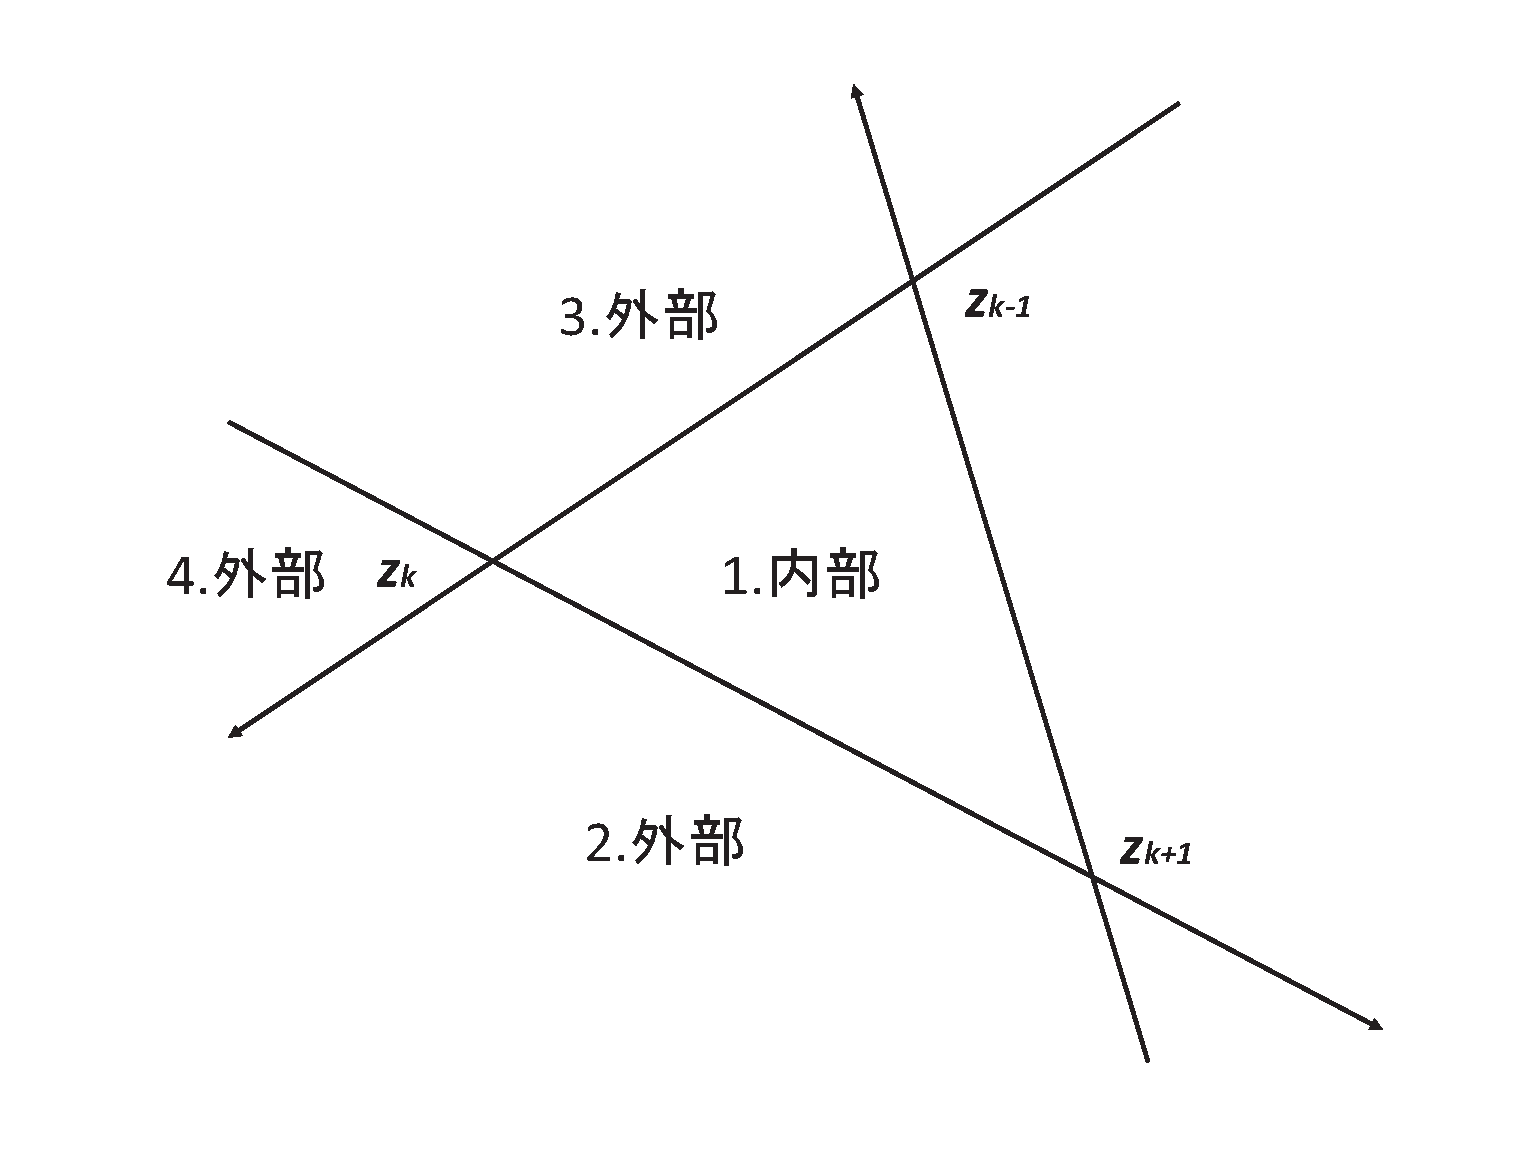
\includegraphics[width=10cm]{hidarimawari_vec.eps} \\
 \vspace{-1mm}
  図4-8. 三点が左回りの三角形
\end{center}

図4-8内の番号は、以下の番号に対応する。
\begin{enumerate}
 \item ベクトル $p z_{k-1}$ と ベクトル $z_{k-1} z_k$ の外積の値が0以上、かつベクトル $p z_k$ とベクトル $z_k z_{k+1}$ の外積の値が0以上ならば内部と判定する。
 \item ベクトル $p z_{k-1}$ と ベクトル $z_{k-1} z_k$ の外積の値が0以上、かつベクトル $p z_k$ とベクトル $z_k z_{k+1}$ の外積の値が負ならば外部と判定する。
 \item ベクトル $p z_{k-1}$ と ベクトル $z_{k-1} z_k$ の外積の値が負であり、かつベクトル $p z_k$ とベクトル $z_k z_{k+1}$ の外積の値が0以上ならば外部と判定する。
 \item ベクトル $p z_{k-1}$ と ベクトル $z_{k-1} z_k$ の外積の値が負であり、かつベクトル $p z_k$ とベクトル $z_k z_{k+1}$ の外積の値が負ならば外部と判定する。
\end{enumerate}

\subsubsection{$z_{k-1},z_k,z_{k+1}$ の三点が、この順番で右回りに三角形を構成している場合}

\begin{center}
  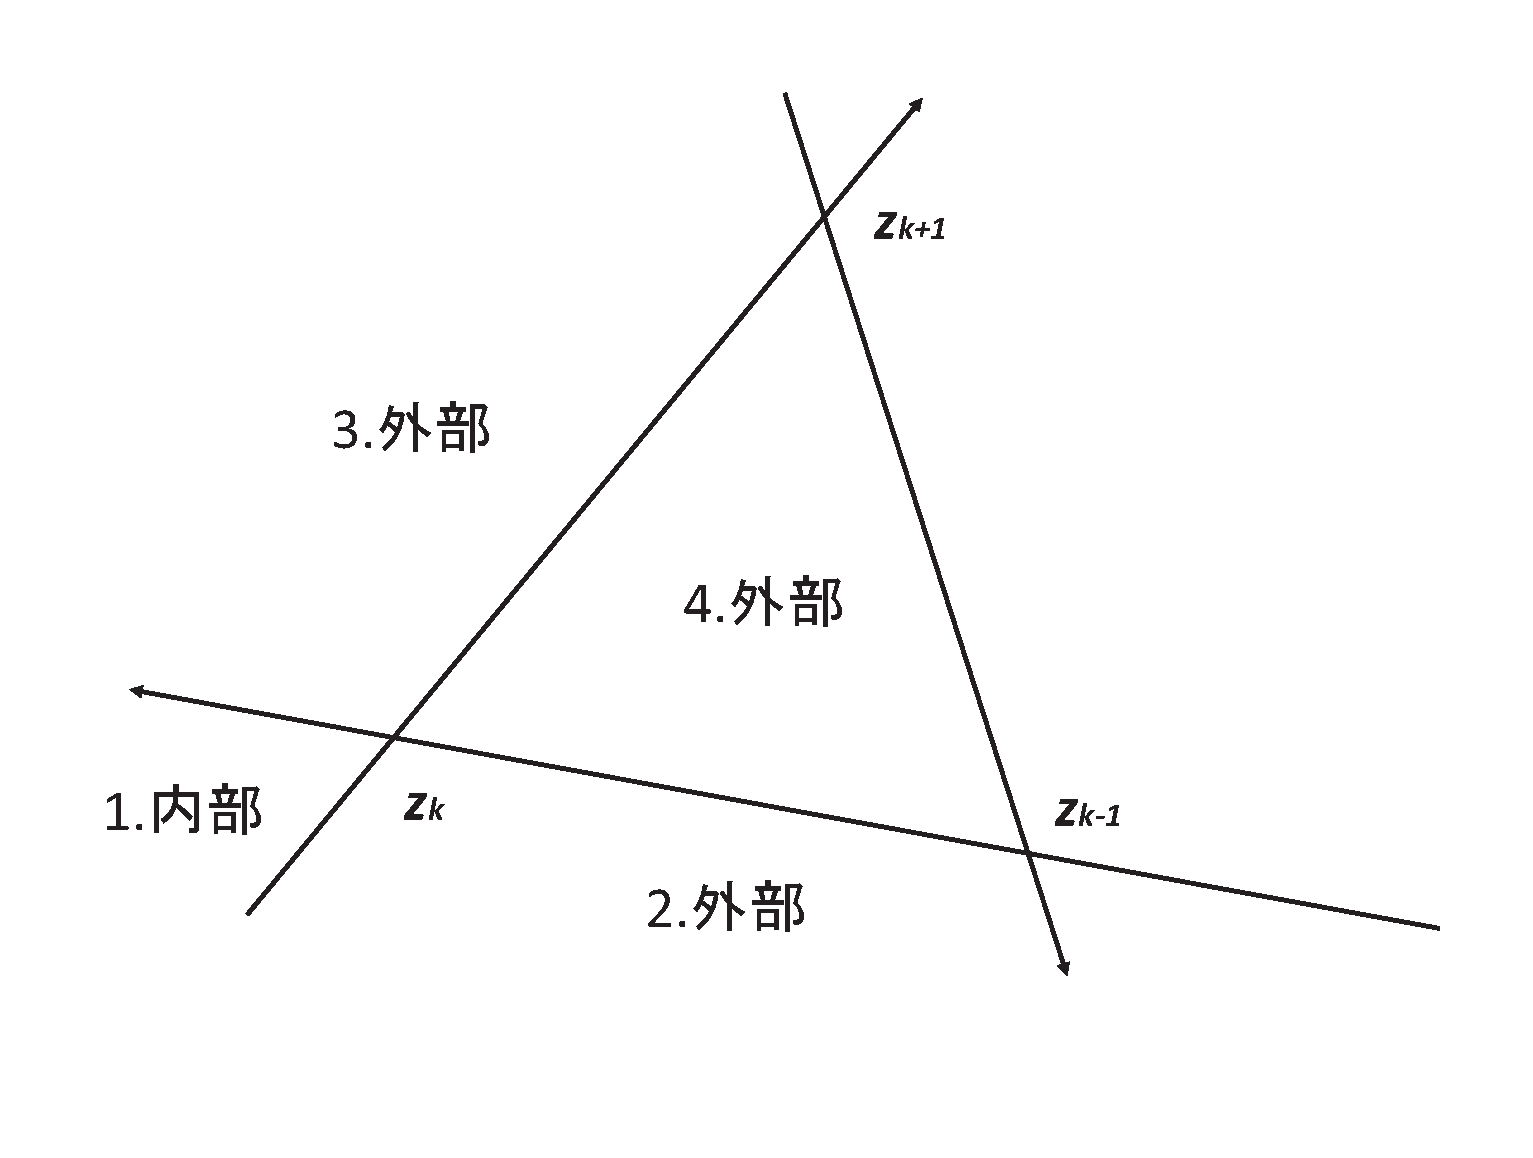
\includegraphics[width=10cm]{migimawari_vec.eps} \\
 \vspace{-1mm}
  図4-9. 三点が右回りの三角形
\end{center}

図4-9内の番号は、以下の番号に対応する。
\begin{enumerate}
 \item ベクトル $p z_{k-1}$ と ベクトル $z_{k-1} z_k$ の外積の値が0以上、かつベクトル $p z_k$ とベクトル $z_k z_{k+1}$ の外積の値が0以上ならば内部と判定する。
 \item ベクトル $p z_{k-1}$ と ベクトル $z_{k-1} z_k$ の外積の値が0以上、かつベクトル $p z_k$ とベクトル $z_k z_{k+1}$ の外積の値が負ならば外部と判定する。
 \item ベクトル $p z_{k-1}$ と ベクトル $z_{k-1} z_k$ の外積の値が負であり、かつベクトル $p z_k$ とベクトル $z_k z_{k+1}$ の外積の値が0以上ならば外部と判定する。
 \item ベクトル $p z_{k-1}$ と ベクトル $z_{k-1} z_k$ の外積の値が負であり、かつベクトル $p z_k$ とベクトル $z_k z_{k+1}$ の外積の値が負ならば外部と判定する。
\end{enumerate}

\subsubsection{$z_{k-1},z_k,z_{k+1}$ の三点が、この順番で右回りに三角形を構成していない場合}

\begin{center}
  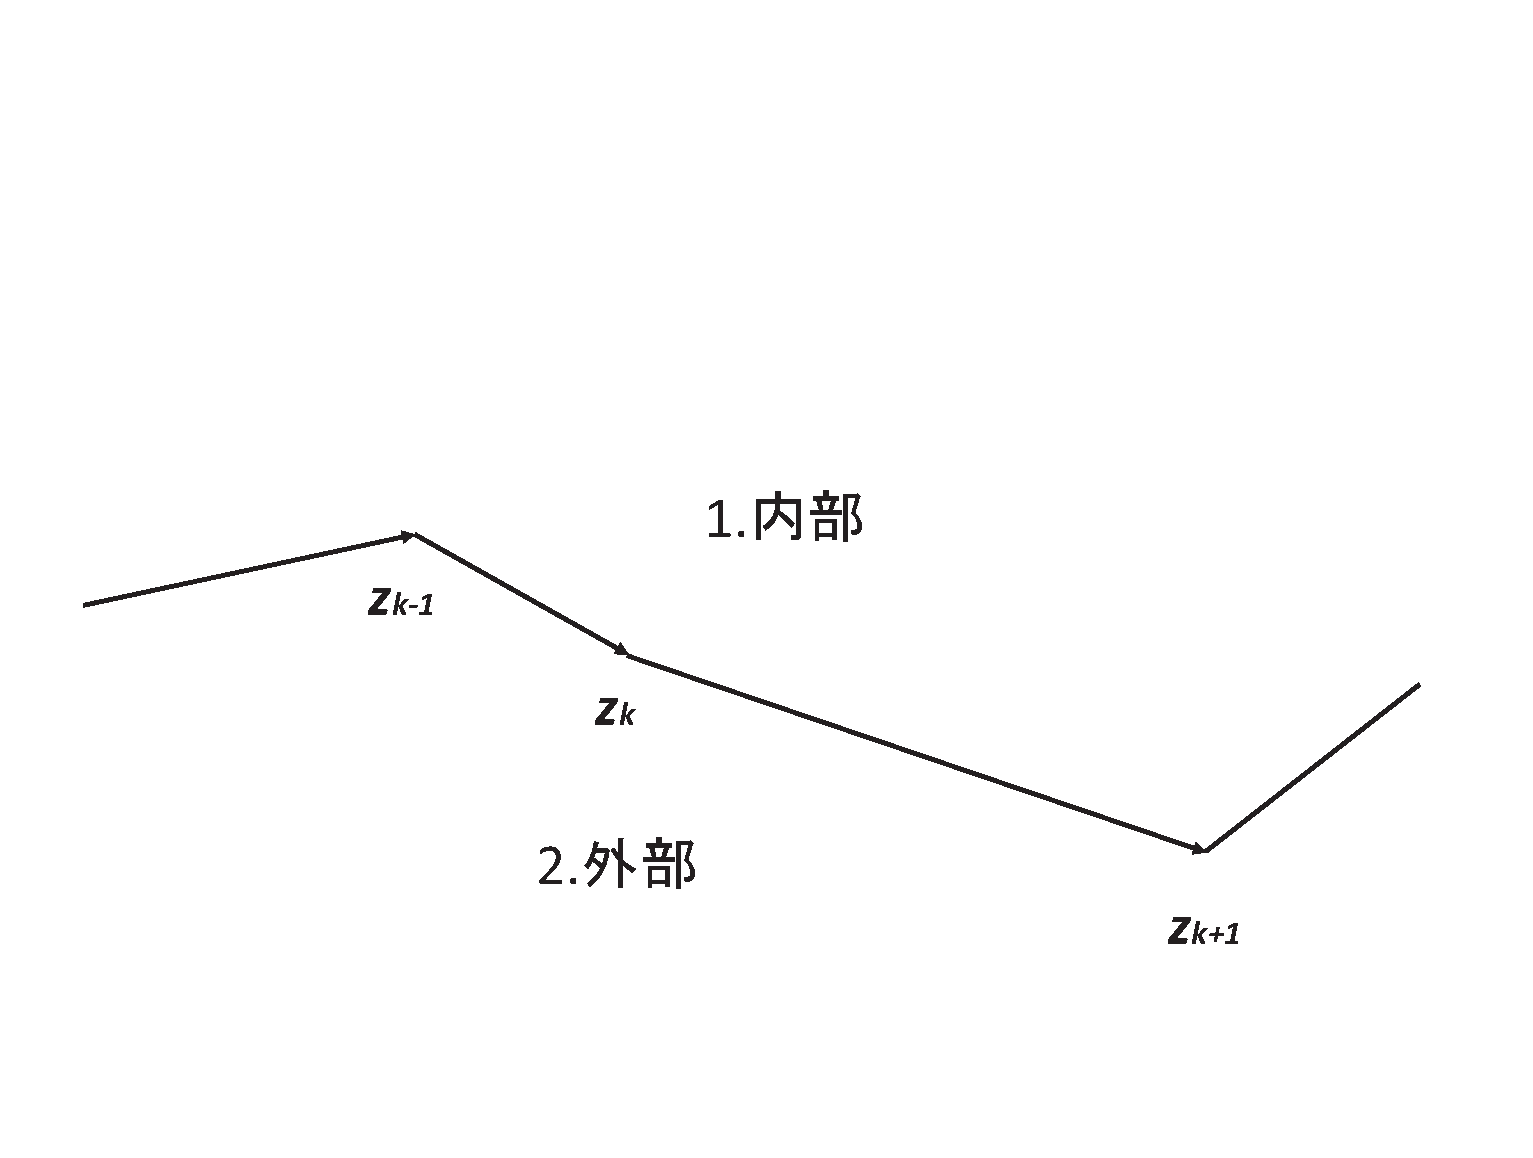
\includegraphics[width=10cm]{sen_vec.eps} \\
 \vspace{-1mm}
  図4-10. 三点が三角形を構成していない
\end{center}

図4-10内の番号は、以下の番号に対応する。
\begin{enumerate}
 \item ベクトル $p z_k$ と ベクトル $z_k z_{k+1}$ の外積の値が0以上ならば内部と判定する。
 \item ベクトル $p z_k$ と ベクトル $z_k z_{k+1}$ の外積の値が負ならば外部と判定する。
\end{enumerate}
この場合、ベクトル $p z_k$ と ベクトル $z_k z_{k+1}$ の外積の値の代わりに、ベクトル $p z_{k-1}$ と ベクトル $z_{k-1} z_k$ の外積の値を用いることも可能である

実際にこのアルゴリズムを使用して、内部外部判定を行った結果が図4-11となる。

\vspace{-5mm}
\begin{center}
  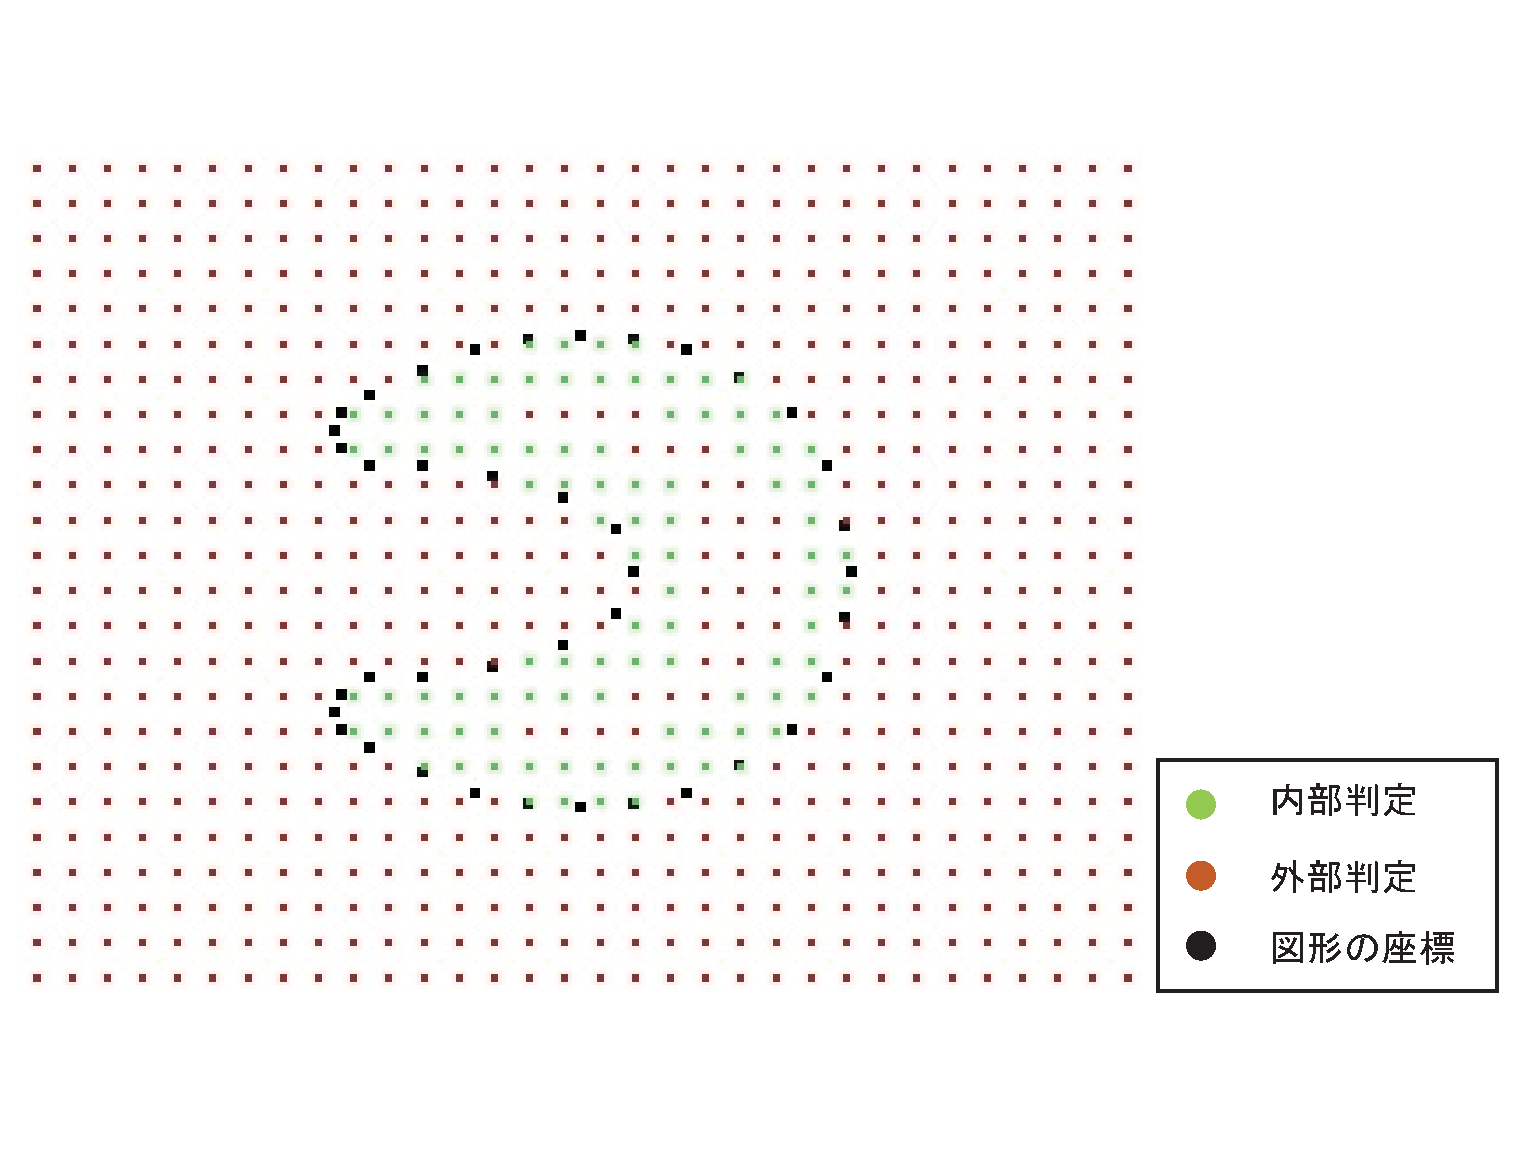
\includegraphics[width=14cm]{Cross_result.eps} \\
 \vspace{-10mm}
  図4-11. 改良版の外積計算による内部外部判定
\end{center}

図を見ると、境界線付近にて正しく判定できていることが分かる。しかしながら、境界線から離れた内部の格子点が正しく判定されていない。

Cauchy の積分定理による方法は、くぼみや穴などを有するドーナッツ型の図形に対する内部外部判定が有利である一方で、複雑形状の図形において、境界線付近での判定に難があるというデメリットが存在する。実際にCauchy の積分定理によって内部外部判定を行った結果が、図4-12となる。

\vspace{-5mm}
\begin{center}
  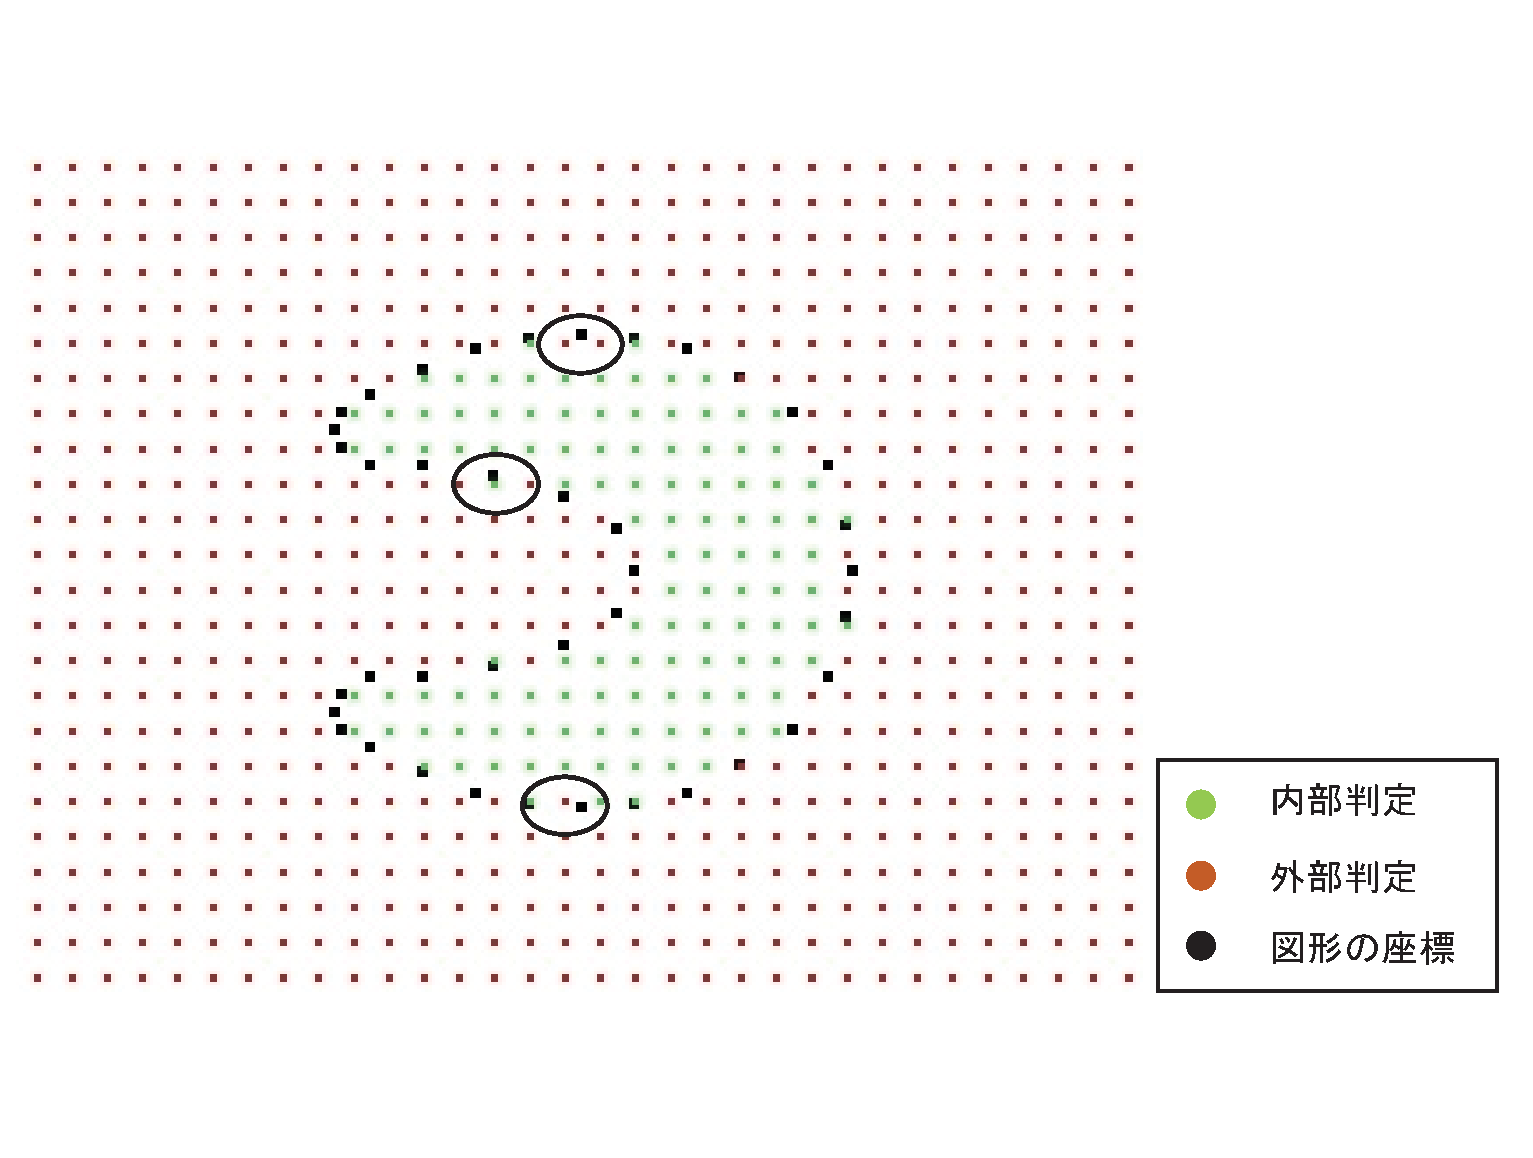
\includegraphics[width=14cm]{Cauchy_result.eps} \\
 \vspace{-10mm}
  図4-12. Cauchyの積分定理による内部外部判定
\end{center}

図を見ると、円で囲まれた格子点が正しく判定されていないことが分かる。

以上の結果を踏まえて、それぞれの方法のデメリットを補うように組み合わせた手法を用いることにする。具体的には、境界線付近の領域では、改良版の外積計算による方法を使用し、境界線から離れた領域では Cauchy の積分定理による方法を使用する。この手法をもとに、内部外部判定を行った結果が、図4-13となる。

\begin{center}
  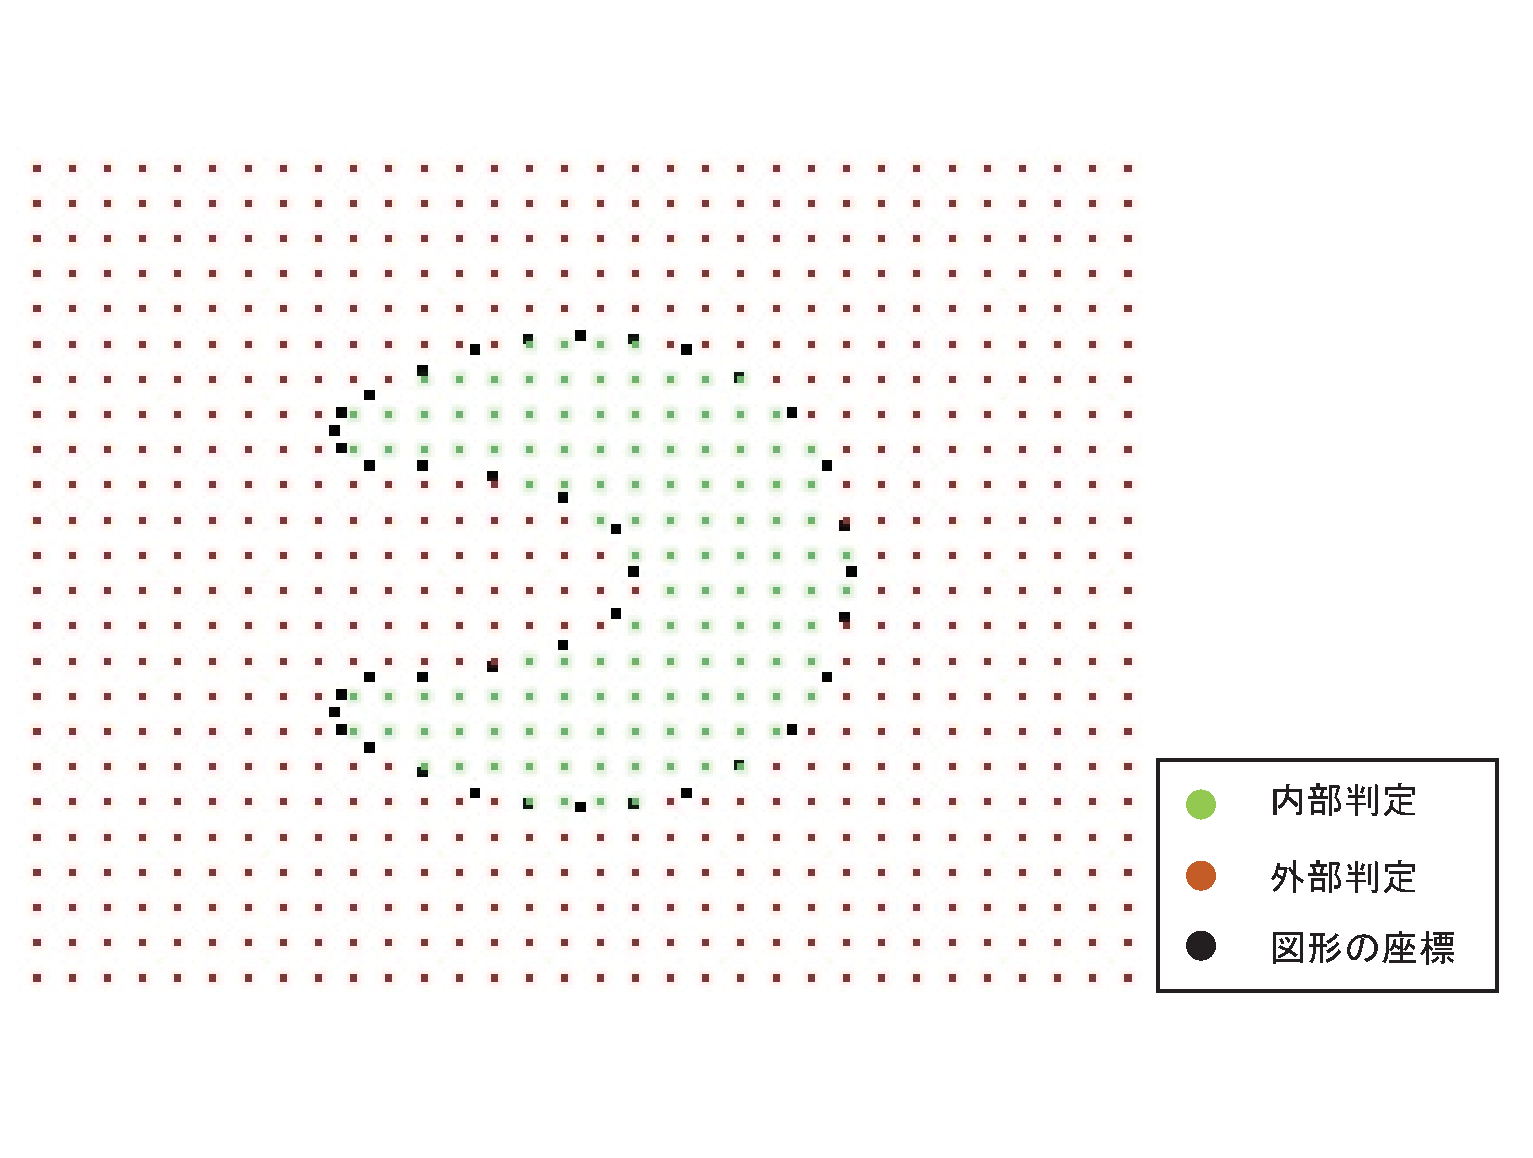
\includegraphics[width=14cm]{Cross-Cauchy_result.eps} \\
 \vspace{-5mm}
  図4-13 外積計算とCauchyの積分定理を組み合わせた判定
\end{center}

改良版の外積計算、および Cauchy の積分定理のそれぞれのデメリットが上手く補われて、すべての格子点について正しく判定されている。同様の処理をすべての階層で行うことで、三次元空間の格子点に対して内部外部判定を行う。


	% アルゴリズム
%\newpage
%% 5
\section{実装}
本システムを構成する、主要な処理について説明する。

% 5.1
\subsection{開発環境}
\begin{center}
  \begin{tabular}{|c|c|}\hline
    \raisebox{-0.2ex}{OS} & \raisebox{-0.2ex}{Windows 8.1 Enterprise 64bit} \\ \hline
    \raisebox{-0.2ex}{CPU} & \raisebox{-0.2ex}{Intel(R) Core(TM) i7-2600 CPU 3.40GHz} \\ \hline
    \raisebox{-0.2ex}{メモリ} & \raisebox{-0.2ex}{4.0GB} \\ \hline
    \raisebox{-0.2ex}{統合開発環境} & \raisebox{-0.2ex}{Unity 5.1.0, Visual Studio Community 2015} \\ \hline
    \raisebox{-0.2ex}{開発言語} & \raisebox{-0.2ex}{C\#} \\ \hline
    \raisebox{-0.2ex}{ライブラリ} & \raisebox{-0.2ex}{OpenCV 2.4.10} \\ \hline
    \raisebox{-0.2ex}{ウェブカメラ} & \raisebox{-0.2ex}{Logicool HD Webcam C270, Logicool HD Webcam C525} \\ \hline
  \end{tabular}
\end{center}

%5.2
\subsection{}
	% 実装
\newpage
% 5
\section{実装}

% 5.1
\subsection{このセクションについて}
原さんの 16 ページからの内容を参考にする	% 実験
\newpage
% 8
\section{謝辞}
感謝	% 総括
\newpage
%%% 8
\section{謝辞}
感謝	% 謝辞
%%\newpage

% 参考文献
%参考文献
\begin{thebibliography}{9}

\bibitem{タグ1}
明石重男, 非凸形状を有する平面図形の形状認識に関するベクトル解析的手法の問題点., 数理解析研究所講究録 第 1544 巻 2007 年 8-12.
\bibitem{タグ2}
児玉賢史, 複雑形状認識の問題点と対処方法, 数理解析研究所講究録, 第 1643 巻 2009 年 148-156.
\bibitem{タグ3}
Inclusion of a Point in a Polygon - Geometry Algorithms,
http://geomalgorithms.com/a03-\_inclusion.html

\end{thebibliography} 
%\newpage

% 付録
%\input{./appendix.tex}
%\newpage

\end{document}


